\documentclass[11pt,a4paper]{article}
\usepackage[utf8]{inputenc}
\usepackage[margin=2.2cm]{geometry}
\usepackage{amsmath,amssymb}
\usepackage{enumitem}
\usepackage{multicol}
\usepackage{array}
\usepackage{booktabs}
\usepackage{pgfplots}
\pgfplotsset{compat=1.18}
\usetikzlibrary{arrows.meta,calc,decorations.markings,patterns}
\usepackage[most]{tcolorbox}
\usepackage{xcolor}
\usepackage{hyperref}
\usepackage{url}
\hypersetup{colorlinks=true,linkcolor=blue!50!black,urlcolor=blue!50!black,
  pdftitle={Física 2.º Bachillerato. Parte 1: herramientas vectoriales, mecánica y gravitación},
  pdfauthor={Jerónimo Arenas García}}
% ---- Datos editables -------------------------------------------------
\newcommand{\autor}{Jerónimo Arenas García}
\newcommand{\repo}{https://github.com/jeroarenas/fisica-2bach-pau}
\newcommand{\version}{v1.0 (noviembre de 2026)}
% ---------------------------------------------------------------------
\setlength{\parindent}{0pt}
\setlength{\parskip}{5pt}

\newcommand{\ii}{\vec{\imath}}
\newcommand{\jj}{\vec{\jmath}}
\newcommand{\kk}{\vec{k}}
\newcommand{\ur}{\vec{u}_r}

\newtcolorbox{clave}[1][]{colback=blue!4,colframe=blue!50!black,fonttitle=\bfseries,title={Idea clave},#1,breakable}
\newtcolorbox{ejemplo}[1][]{colback=green!3,colframe=green!40!black,fonttitle=\bfseries,title={Ejemplo},#1,breakable}
\newtcolorbox{ojo}[1][]{colback=orange!6,colframe=orange!70!black,fonttitle=\bfseries,title={Ojo},#1,breakable}

\renewcommand{\contentsname}{Índice}

\begin{document}

\begin{titlepage}
\centering
\vspace*{0.3cm}
{\huge\bfseries Física 2.º Bachillerato\par}
\vspace{0.4cm}
{\Large Parte 1: herramientas vectoriales, mecánica\\[2pt] e interacción gravitatoria\par}
\vspace{0.4cm}
{\normalsize Apuntes autocontenidos con deducciones, ejemplos resueltos\\ y problemas graduados tipo PAU\par}
\vspace{0.4cm}
{\large \autor\par}
\vspace{0.3cm}
{\normalsize \version\par}
\vspace{0.2cm}
{\small \url{\repo}\par}
\vspace{0.4cm}
\begin{tcolorbox}[colback=blue!4,colframe=blue!50!black,fonttitle=\bfseries,title={A quién va dirigido},halign=left,width=\textwidth]
\small
A quien tiene base técnica y necesita \textbf{ponerse al día rápido} con la Física de 2.º de Bachillerato: madres y padres que quieren ayudar a sus hijos con la PAU, profesores particulares, docentes de otras materias o universitarios que dan clases. También a estudiantes avanzados que no quieren quedarse con fórmulas ``mágicas''. No avanza paso a paso como un libro de texto: es un material de referencia breve, en el que cada fórmula se deduce o se justifica, con ejemplos resueltos y problemas para practicar con el estudiante.

\smallskip
\textbf{Alcance.} Cubre los contenidos habituales del primer trimestre: herramientas matemáticas (vectores), cinemática y dinámica de la partícula, momento angular, leyes de Kepler, gravitación, energía y campo gravitatorio. No sustituye al libro de texto ni a las indicaciones del profesorado: conviene contrastar notación y criterios con los de la PAU de cada comunidad autónoma.
\end{tcolorbox}

\begin{tcolorbox}[colback=gray!4,colframe=gray!60!black,fonttitle=\bfseries,title={Licencia},halign=left,width=\textwidth]
\small
Este documento se distribuye bajo la licencia \textbf{Creative Commons Reconocimiento-NoComercial-CompartirIgual 4.0 Internacional (CC BY-NC-SA 4.0)}: \url{https://creativecommons.org/licenses/by-nc-sa/4.0/deed.es}.

Puedes copiarlo, redistribuirlo y adaptarlo libremente, siempre que (1) cites la autoría y enlaces la fuente, (2) no lo uses con fines comerciales y (3) compartas tus versiones derivadas con la misma licencia.

\textbf{Cómo citar:} \autor, \emph{Física 2.º Bachillerato. Parte 1: herramientas vectoriales, mecánica e interacción gravitatoria}, \version. \url{\repo}.
\end{tcolorbox}

\begin{tcolorbox}[colback=gray!4,colframe=gray!60!black,fonttitle=\bfseries,title={Cómo se ha elaborado este documento},halign=left,width=\textwidth]
\small
Estos apuntes nacieron preparando con una estudiante la Física de 2.º de Bachillerato. Se han redactado con la ayuda de \textbf{Claude} (un asistente de inteligencia artificial de Anthropic), que generó borradores de texto, figuras, ejemplos y problemas a partir de las indicaciones, preguntas y correcciones del autor. Todo el contenido ha sido revisado por el autor, y los resultados numéricos de ejemplos y problemas se han comprobado por cálculo.

Aun así, puede contener errores. Si encuentras alguno, o tienes sugerencias, abre una \emph{issue} o una \emph{pull request} en el repositorio.
\end{tcolorbox}




\end{titlepage}

\tableofcontents

%=====================================================================
\section{Magnitudes y unidades}
%=====================================================================
Una \textbf{magnitud física} es cualquier propiedad que se puede medir. Hay dos tipos:
\begin{itemize}[itemsep=2pt]
  \item \textbf{Escalares}: quedan definidas con un número y su unidad. Ejemplos: tiempo $t$, masa $m$, energía $E$, trabajo $W$.
  \item \textbf{Vectoriales}: además del número (\emph{módulo}) necesitan \emph{dirección} y \emph{sentido}. Ejemplos: velocidad $\vec v$, fuerza $\vec F$, campo gravitatorio $\vec g$.
\end{itemize}

\textbf{Sistema Internacional (SI).} Unidades básicas que usaremos: metro (m), kilogramo (kg), segundo (s), mol, amperio (A), kelvin (K). Las demás son \emph{derivadas}; por ejemplo, la frecuencia $f=\frac1T$ se mide en $\mathrm{s^{-1}}=\mathrm{Hz}$ y la velocidad en $\mathrm{m/s}=\mathrm{m\cdot s^{-1}}$. El newton es $1\ \mathrm{N}=1\ \mathrm{kg\cdot m/s^2}$ y el julio $1\ \mathrm J=1\ \mathrm{N\cdot m}$.

\textbf{Notación científica y prefijos.} Los resultados se dan como $d_1{,}d_2\ldots\cdot10^{n}$. Prefijos habituales: tera ($10^{12}$), giga ($10^9$), mega ($10^6$), kilo ($10^3$), hecto ($10^2$), deca ($10$), deci ($10^{-1}$), centi ($10^{-2}$), mili ($10^{-3}$), micro ($10^{-6}$), nano ($10^{-9}$), pico ($10^{-12}$).

\begin{ojo}
En los problemas de gravitación casi todo hay que pasarlo al SI antes de operar: km $\to$ m, horas/días/años $\to$ s. Un año son $365\cdot24\cdot3600\approx3{,}156\cdot10^7$ s. Es la fuente de error más frecuente.
\end{ojo}

%=====================================================================
\section{Cálculo vectorial}
%=====================================================================
\subsection{Componentes, módulo y ángulo}
En el plano, un vector se escribe con sus componentes respecto a los vectores unitarios $\ii=(1,0)$ y $\jj=(0,1)$ (en el espacio se añade $\kk=(0,0,1)$):
\[
\vec v=(v_x,v_y)=v_x\,\ii+v_y\,\jj .
\]
\begin{minipage}{0.55\textwidth}
\begin{itemize}[itemsep=2pt]
  \item \textbf{Módulo} (``intensidad''): $|\vec v|=\sqrt{v_x^2+v_y^2}$ \ (en 3D se suma $v_z^2$).
  \item \textbf{Dirección}: la recta que contiene al vector. \textbf{Sentido}: hacia dónde apunta la flecha.
  \item \textbf{Ángulo} con el eje $X$ positivo: $\tan\alpha=\dfrac{v_y}{v_x}$.
  \item Al revés, si conocemos módulo y ángulo:
  \[ v_x=|\vec v|\cos\alpha,\qquad v_y=|\vec v|\sin\alpha. \]
\end{itemize}
\end{minipage}\hfill
\begin{minipage}{0.4\textwidth}
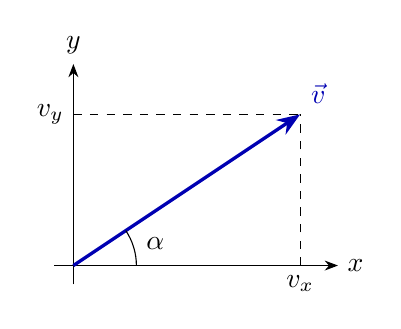
\begin{tikzpicture}[scale=0.8,>=Stealth]
  \draw[->] (-0.3,0)--(4.2,0) node[right]{$x$};
  \draw[->] (0,-0.3)--(0,3.2) node[above]{$y$};
  \draw[->,very thick,blue!70!black] (0,0)--(3.6,2.4) node[above right]{$\vec v$};
  \draw[dashed] (3.6,0)--(3.6,2.4) (0,2.4)--(3.6,2.4);
  \node[below] at (3.6,0) {$v_x$}; \node[left] at (0,2.4) {$v_y$};
  \draw (1,0) arc (0:33.7:1); \node at (1.3,0.35) {$\alpha$};
\end{tikzpicture}
\end{minipage}

\begin{ojo}[title={Ojo con el cuadrante}]
La calculadora da $\arctan$ entre $-90^\circ$ y $90^\circ$ y \emph{no distingue cuadrantes}. Hay que mirar los signos de las componentes. Para $\vec F=(-4,-3)$ N: $\arctan\frac{-3}{-4}=36{,}87^\circ$, pero el vector está en el \textbf{tercer cuadrante}, así que $\alpha=180^\circ+36{,}87^\circ=216{,}87^\circ$. (Error frecuente: dar $37^\circ$, que es el ángulo con el eje, no el argumento.)
\end{ojo}

\subsection{Operaciones básicas}
\begin{itemize}[itemsep=2pt]
  \item \textbf{Suma y resta} (componente a componente): $\vec u\pm\vec v=(u_x\pm v_x,\ u_y\pm v_y)$. Gráficamente, la suma es la diagonal del paralelogramo (o se colocan ``punta con cola''); restar es sumar el opuesto, $\vec u-\vec v=\vec u+(-\vec v)$.
  \item \textbf{Producto por un escalar}: $k\,\vec v=(k v_x,k v_y)$. Si $k>0$ conserva el sentido; si $k<0$ lo invierte; el módulo queda multiplicado por $|k|$.
\end{itemize}

\begin{ejemplo}[title={Ejemplo: suma de tres vectores}]
$|\vec u|=8$ m a $150^\circ$, \ $|\vec v|=15$ m a $45^\circ$, \ $|\vec w|=20$ m a $240^\circ$.
\begin{enumerate}[itemsep=1pt]
  \item Componentes: $\vec u=(-6{,}93;\,4{,}00)$, \ $\vec v=(10{,}61;\,10{,}61)$, \ $\vec w=(-10{,}00;\,-17{,}32)$ m.
  \item Suma: $\vec s=(-6{,}32;\,-2{,}71)$ m. \ Módulo: $|\vec s|=\sqrt{6{,}32^2+2{,}71^2}=6{,}88$ m.
  \item Ángulo: $\arctan\frac{-2{,}71}{-6{,}32}=23{,}2^\circ$, pero las dos componentes son negativas (3.\textsuperscript{er} cuadrante): $\alpha=180^\circ+23{,}2^\circ=203{,}2^\circ$.
\end{enumerate}
\end{ejemplo}

\subsection{Producto escalar}
\[
\boxed{\ \vec u\cdot\vec v=|\vec u|\,|\vec v|\cos\alpha=u_xv_x+u_yv_y+u_zv_z\ }
\]
El resultado es un \textbf{número} (escalar), no un vector. Mide cuánto ``apunta'' un vector en la dirección del otro: $|\vec v|\cos\alpha$ es la proyección de $\vec v$ sobre $\vec u$.

Propiedades:
\begin{enumerate}[itemsep=1pt]
  \item Es conmutativo: $\vec u\cdot\vec v=\vec v\cdot\vec u$.
  \item Si $\vec u\perp\vec v$ ($\alpha=90^\circ$): $\vec u\cdot\vec v=0$. \ (Es el test de perpendicularidad.)
  \item Si $\vec u\parallel\vec v$ con el mismo sentido ($\alpha=0^\circ$): $\vec u\cdot\vec v=|\vec u|\,|\vec v|$. En particular $\vec v\cdot\vec v=|\vec v|^2$.
\end{enumerate}
\textbf{Uso principal}: calcular el ángulo entre dos vectores, $\cos\alpha=\dfrac{\vec u\cdot\vec v}{|\vec u|\,|\vec v|}$. \textbf{En física}: el trabajo de una fuerza constante es $W=\vec F\cdot\Delta\vec r=|\vec F|\,|\Delta\vec r|\cos\alpha$.

\begin{ejemplo}
$\vec u=\ii-2\jj+4\kk$, \ $\vec v=3\ii+\jj-\kk$.
$\vec u\cdot\vec v=1\cdot3+(-2)\cdot1+4\cdot(-1)=-3$; \ $|\vec u|=\sqrt{21}=4{,}58$; \ $|\vec v|=\sqrt{11}=3{,}32$.
$\cos\alpha=\frac{-3}{15{,}20}=-0{,}197\Rightarrow\alpha=101{,}4^\circ$. (El signo negativo indica que el ángulo es obtuso.)
\end{ejemplo}

\subsection{Producto vectorial}
El producto vectorial $\vec u\times\vec v$ es \textbf{otro vector} $\vec p$ definido por:
\begin{itemize}[itemsep=2pt]
  \item \textbf{Módulo}: $|\vec u\times\vec v|=|\vec u|\,|\vec v|\sin\alpha$. \ Coincide con el \emph{área del paralelogramo} que forman $\vec u$ y $\vec v$.
  \item \textbf{Dirección}: perpendicular al plano que forman $\vec u$ y $\vec v$.
  \item \textbf{Sentido}: regla de la mano derecha (o del sacacorchos). Si al girar de $\vec u$ hacia $\vec v$ por el ángulo más corto el giro se ve \emph{antihorario}, el producto sale hacia nosotros ($\odot$); si se ve \emph{horario}, entra en el papel ($\otimes$).
\end{itemize}

\begin{center}
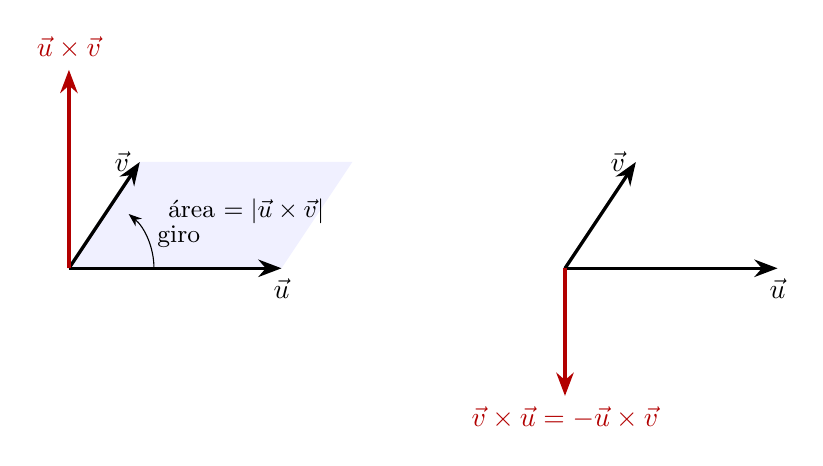
\begin{tikzpicture}[>=Stealth,scale=0.9]
  \fill[blue!6] (0,0)--(3,0)--(4,1.5)--(1,1.5)--cycle;
  \draw[->,very thick] (0,0)--(3,0) node[below]{$\vec u$};
  \draw[->,very thick] (0,0)--(1,1.5) node[left]{$\vec v$};
  \draw[->,very thick,red!70!black] (0,0)--(0,2.8) node[above]{$\vec u\times\vec v$};
  \draw[->] (1.2,0) arc (0:50:1.0); \node at (1.55,0.45){\small giro};
  \node at (2.5,0.8) {\small área $=|\vec u\times\vec v|$};
  \begin{scope}[xshift=7cm]
  \draw[->,very thick] (0,0)--(3,0) node[below]{$\vec u$};
  \draw[->,very thick] (0,0)--(1,1.5) node[left]{$\vec v$};
  \draw[->,very thick,red!70!black] (0,0)--(0,-1.8) node[below]{$\vec v\times\vec u=-\vec u\times\vec v$};
  \end{scope}
\end{tikzpicture}
\end{center}

Propiedades:
\begin{enumerate}[itemsep=1pt]
  \item \textbf{No es conmutativo}: $\vec v\times\vec u=-(\vec u\times\vec v)$. El orden importa.
  \item Si $\vec u\perp\vec v$: $\sin90^\circ=1\Rightarrow|\vec u\times\vec v|=|\vec u|\,|\vec v|$ (valor máximo).
  \item Si $\vec u\parallel\vec v$ ($\alpha=0^\circ$ o $180^\circ$): $\sin\alpha=0\Rightarrow\vec u\times\vec v=\vec 0$.
  \item Unitarios: $\ii\times\jj=\kk$, \ $\jj\times\kk=\ii$, \ $\kk\times\ii=\jj$ (orden cíclico); al revés, signo menos.
\end{enumerate}

\textbf{Cálculo por determinante} (se desarrolla por la primera fila; ¡el término de $\jj$ lleva signo menos!):
\[
\vec a\times\vec b=\begin{vmatrix}\ii&\jj&\kk\\ a_1&a_2&a_3\\ b_1&b_2&b_3\end{vmatrix}
=\ii\begin{vmatrix}a_2&a_3\\ b_2&b_3\end{vmatrix}
-\jj\begin{vmatrix}a_1&a_3\\ b_1&b_3\end{vmatrix}
+\kk\begin{vmatrix}a_1&a_2\\ b_1&b_2\end{vmatrix}.
\]

\begin{ejemplo}
\textbf{a)} $\vec c=-\ii+3\jj+2\kk$, \ $\vec d=2\ii-\jj+4\kk$:
\[
\vec c\times\vec d=\ii\,[3\cdot4-2\cdot(-1)]-\jj\,[(-1)\cdot4-2\cdot2]+\kk\,[(-1)(-1)-3\cdot2]=14\ii+8\jj-5\kk .
\]
\textbf{b)} $\vec a=2\ii+3\jj$, \ $\vec b=-\ii+4\jj$ (ambos en el plano $XY$): $\vec a\times\vec b=\kk\,[2\cdot4-3\cdot(-1)]=11\kk$.
Sale en la dirección $\kk$, perpendicular al plano $XY$, como debe ser. El paralelogramo que forman tiene área 11.
\end{ejemplo}

\subsection{Momento de un vector respecto a un punto}
Dado un vector $\vec v$ aplicado en un punto $P$, y un punto de referencia $O$, el \textbf{momento} de $\vec v$ respecto a $O$ es
\[
\boxed{\ \vec M_O=\vec r\times\vec v\ }\qquad \vec r=\overrightarrow{OP}\ \text{(vector de posición de $P$ respecto a $O$)}.
\]
Es una magnitud vectorial. Su módulo es $|\vec M_O|=r\,v\sin\alpha=v\cdot d$, donde $\alpha$ es el ángulo entre $\vec r$ y $\vec v$ y $d=r\sin\alpha$ es la \emph{distancia de $O$ a la recta de acción} de $\vec v$ (el ``brazo''). Mide la tendencia a \emph{girar} alrededor de $O$. Su dirección es perpendicular al plano que forman $\vec r$ y $\vec v$, y su sentido lo da la regla de la mano derecha.

\begin{center}
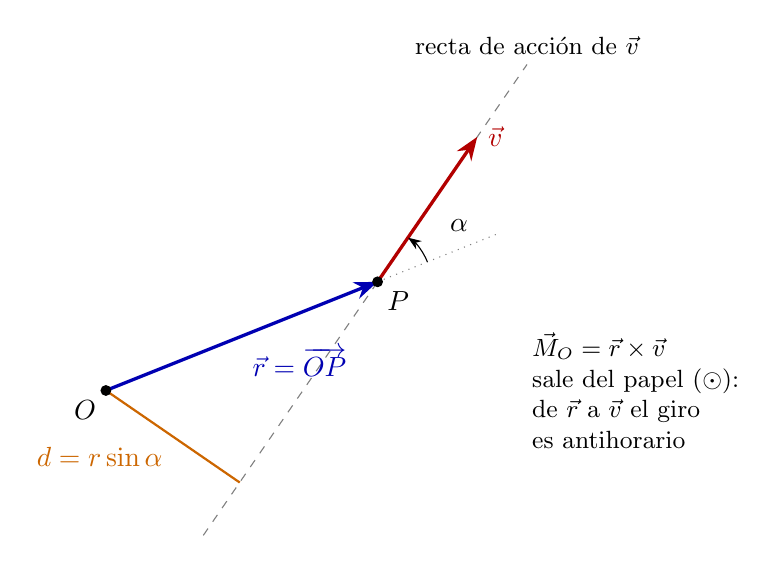
\begin{tikzpicture}[>=Stealth,scale=1.15]
  \coordinate (O) at (0,0);
  \coordinate (P) at (3,1.2);
  \coordinate (V) at ($(P)+(1.1,1.6)$);
  \coordinate (B) at ($(P)-1.75*(1.1,1.6)$);
  \coordinate (H) at ($(B)!(O)!(V)$);
  % recta de acción
  \draw[dashed,gray] (B)--($(P)+1.5*(1.1,1.6)$) node[above,black]{\small recta de acción de $\vec v$};
  % prolongación de r para el ángulo
  \draw[dotted,gray] (P)--($(P)!0.45!($(P)+(3,1.2)$)$);
  % brazo d
  \draw[thick,orange!80!black] (O)--(H) node[midway,below left]{$d=r\sin\alpha$};
  \draw[orange!80!black] let \p1=($(O)-(H)$), \p2=($(V)-(H)$) in
      ($(H)+0.18*({\x1/veclen(\x1,\y1)},{\y1/veclen(\x1,\y1)})$) --
      ($(H)+0.18*({\x1/veclen(\x1,\y1)},{\y1/veclen(\x1,\y1)})+0.18*({\x2/veclen(\x2,\y2)},{\y2/veclen(\x2,\y2)})$) --
      ($(H)+0.18*({\x2/veclen(\x2,\y2)},{\y2/veclen(\x2,\y2)})$);
  % vectores
  \draw[->,very thick,blue!70!black] (O)--(P) node[midway,below right]{$\vec r=\overrightarrow{OP}$};
  \draw[->,very thick,red!70!black] (P)--(V) node[right]{$\vec v$};
  % ángulo alfa entre la prolongación de r y v
  \draw[->] ($(P)+(0.55,0.22)$) arc[start angle=21.8,end angle=55.5,radius=0.59];
  \node at ($(P)+(0.9,0.62)$) {$\alpha$};
  % puntos
  \fill (O) circle (0.06) node[below left]{$O$};
  \fill (P) circle (0.06) node[below right]{$P$};
  \node[anchor=west,align=left,font=\small] at (4.6,0.0) {$\vec M_O=\vec r\times\vec v$\\ sale del papel ($\odot$):\\ de $\vec r$ a $\vec v$ el giro\\ es antihorario};
\end{tikzpicture}
\end{center}

Según qué vector sea $\vec v$, el momento tiene distintos nombres y significados:
\begin{itemize}[itemsep=2pt]
  \item $\vec r\times\vec F$: \textbf{momento de una fuerza} (N·m). Es lo que hace girar una llave inglesa: más fuerza o más brazo, más efecto (ver el ejemplo de abajo).
  \item $\vec r\times\vec v$: \textbf{momento de la velocidad} (m$^2$/s). Su módulo es el doble del área que barre $\vec r$ por segundo (velocidad areolar, ver §\ref{sec:areolar}).
  \item $\vec r\times m\vec v=\vec r\times\vec p$: \textbf{momento angular} (kg·m$^2$/s), ver §\ref{sec:L}.
\end{itemize}

\begin{ejemplo}[title={Ejemplo: la llave inglesa (momento de una fuerza)}]
Apretamos una tuerca $O$ con la misma fuerza $F=50$ N, siempre perpendicular a la llave ($\alpha=90^\circ$, $\sin\alpha=1$), con dos llaves de distinta longitud:
\begin{center}
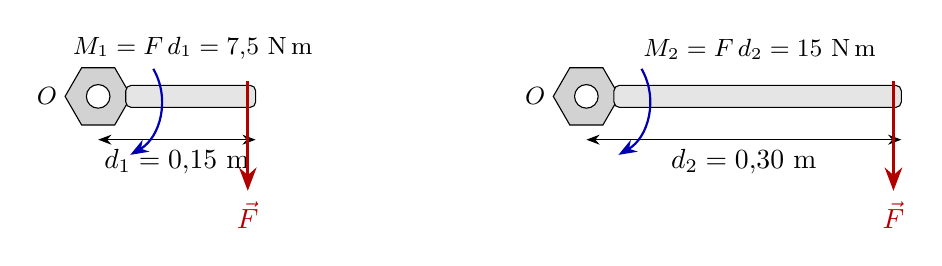
\begin{tikzpicture}[>=Stealth,scale=1.0]
  \foreach \xo/\L/\lab/\mom in {0/2/{d_1=0{,}15\ \mathrm m}/{M_1=F\,d_1=7{,}5\ \mathrm{N\,m}}, 6.2/4/{d_2=0{,}30\ \mathrm m}/{M_2=F\,d_2=15\ \mathrm{N\,m}}}{
    \begin{scope}[xshift=\xo cm]
      \fill[gray!35,draw=black] (0:0.42) \foreach \a in {60,120,...,300}{--(\a:0.42)}--cycle;
      \fill[white,draw=black] (0,0) circle (0.15);
      \fill[gray!20,draw=black,rounded corners=2pt] (0.35,-0.14) rectangle (\L,0.14);
      \draw[<->] (0,-0.55)--(\L,-0.55) node[midway,below]{$\lab$};
      \draw[->,very thick,red!70!black] (\L-0.1,0.2)--(\L-0.1,-1.2) node[below]{$\vec F$};
      \draw[->,thick,blue!70!black] (0.7,0.35) arc[start angle=30,end angle=-60,radius=0.8];
      \node[anchor=south,font=\small] at (\L/2+0.2,0.35) {$\mom$};
      \node[font=\small] at (-0.65,0) {$O$};
    \end{scope}}
\end{tikzpicture}
\end{center}
\begin{itemize}[itemsep=2pt]
  \item Con la misma fuerza, la llave el doble de larga produce \textbf{el doble de momento}. Por eso cuesta menos aflojar una tuerca con una llave larga: para conseguir el mismo momento basta la mitad de fuerza.
  \item \textbf{Qué significa ``más momento''.} El momento es a los giros lo que la fuerza a los desplazamientos. Igual que una fuerza mayor hace aumentar más deprisa la velocidad ($\vec F=\frac{d\vec p}{dt}$), un momento mayor hace aumentar más deprisa la velocidad de giro, en el sentido en que empuja la fuerza ($\vec M=\frac{d\vec L}{dt}$, ver §\ref{sec:L}). Con la llave larga, la tuerca (si está suelta) empieza a girar más deprisa en el mismo tiempo.
  \item \textbf{Sentido}: en la figura, la fuerza hace girar la llave en sentido \emph{horario}, así que $\vec M$ entra en el papel ($\otimes$).
  \item Si empujamos la llave \emph{a lo largo de su mango}, hacia la tuerca ($\alpha=0^\circ$), el momento es nulo y no gira, por mucha fuerza que hagamos: solo cuenta la componente de la fuerza perpendicular al brazo.
\end{itemize}
\end{ejemplo}

\begin{ejemplo}[title={Ejemplo: momento de la velocidad}]
Una partícula está en $\vec r=3\ii-\jj+2\kk$ (m) y se mueve con $\vec v=\ii+2\jj-3\kk$ (m/s).
\[
\vec M=\begin{vmatrix}\ii&\jj&\kk\\3&-1&2\\1&2&-3\end{vmatrix}
=\ii(3-4)-\jj(-9-2)+\kk(6+1)=-\ii+11\jj+7\kk\ \ \mathrm{m^2/s}.
\]
\end{ejemplo}

%=====================================================================
\section{Cinemática}
%=====================================================================
La cinemática \emph{describe} el movimiento sin preocuparse de sus causas.

\subsection{Vector de posición, ecuaciones del movimiento y trayectoria}
Fijado un \textbf{sistema de referencia} (origen $O$ y ejes), la posición de la partícula en cada instante es
\[
\vec r(t)=x(t)\,\ii+y(t)\,\jj+z(t)\,\kk\quad(\mathrm m),\qquad |\vec r|=\text{distancia al origen}.
\]
Las funciones $x(t)$, $y(t)$, $z(t)$ son las \textbf{ecuaciones (paramétricas) del movimiento}.

La \textbf{trayectoria} es la línea que recorre la partícula. En 2D se obtiene \emph{eliminando $t$} entre $x(t)$ e $y(t)$.

\subsection{Desplazamiento, velocidad y aceleración}
\begin{itemize}[itemsep=3pt]
  \item \textbf{Vector desplazamiento}: $\Delta\vec r=\vec r_f-\vec r_0$. Une la posición inicial con la final; no depende del camino.
  \item \textbf{Velocidad media}: $\vec v_m=\dfrac{\Delta\vec r}{\Delta t}$. Tiene la dirección de $\Delta\vec r$ (secante a la trayectoria).
  \item \textbf{Velocidad instantánea}: $\vec v(t)=\dfrac{d\vec r}{dt}=\vec r\,'(t)$. Es \emph{tangente} a la trayectoria. Su módulo $|\vec v|$ es la \textbf{rapidez}.
  \item \textbf{Aceleración media}: $\vec a_m=\dfrac{\Delta\vec v}{\Delta t}$. \quad \textbf{Instantánea}: $\vec a(t)=\dfrac{d\vec v}{dt}=\vec v\,'(t)=\vec r\,''(t)$ \ (m/s$^2$).
\end{itemize}

\begin{clave}
Posición $\xrightarrow{\ \text{derivar}\ }$ velocidad $\xrightarrow{\ \text{derivar}\ }$ aceleración. Se deriva cada componente por separado.
\end{clave}

\begin{ejemplo}[title={Ejemplo: $\vec r(t)=2t\,\ii+(t^2+1)\,\jj+3\kk$ (m)}]
\begin{itemize}[itemsep=2pt]
  \item Ecuaciones: $x=2t$, \ $y=t^2+1$, \ $z=3$ (el movimiento ocurre en el plano $z=3$).
  \item Trayectoria: $t=\frac x2\Rightarrow y=\left(\frac x2\right)^2+1=\frac14x^2+1$ (una parábola).
  \item Desplazamiento entre $t=0$ y $t=2$ s: $\vec r_0=\jj+3\kk$, \ $\vec r_2=4\ii+5\jj+3\kk$ $\Rightarrow\Delta\vec r=4\ii+4\jj$ m.
  \item Velocidad media: $\vec v_m=\frac{4\ii+4\jj}{2}=2\ii+2\jj$ m/s.
  \item Velocidad instantánea: $\vec v(t)=2\ii+2t\,\jj$ m/s. Por ejemplo, $\vec v(0)=2\ii$, \ $\vec v(1)=2\ii+2\jj$ m/s ($|\vec v(1)|=2\sqrt2=2{,}83$ m/s).
  \item Aceleración: $\vec a(t)=\vec v\,'(t)=2\jj$ m/s$^2$: \textbf{constante}.
\end{itemize}
\end{ejemplo}

\begin{ojo}
Error frecuente: derivar una sola vez y llamar ``aceleración'' a lo que sale. Al derivar $\vec r(t)$ se obtiene la \emph{velocidad}; hay que derivar otra vez para la aceleración. Si, como aquí, la aceleración es constante, coincide con la aceleración media en cualquier intervalo.
\end{ojo}

\subsection{Componentes intrínsecas de la aceleración}\label{sec:intr}
En lugar de los ejes $X,Y$, se puede descomponer la aceleración según la propia trayectoria, en cada punto: una parte \textbf{tangente} (en la dirección de $\vec v$, vector unitario $\vec u_t=\vec v/v$) y otra \textbf{normal} (perpendicular a la anterior, hacia el centro de la curva, vector unitario $\vec u_n$):
\[
\vec a=a_t\,\vec u_t+a_n\,\vec u_n,\qquad a_t=\frac{dv}{dt},\qquad a_n=\frac{v^2}{R},\qquad |\vec a|=\sqrt{a_t^2+a_n^2}.
\]
Notación: aquí $v=|\vec v|$ es el \textbf{módulo de la velocidad} (la rapidez, en m/s) y $R$ es el \textbf{radio de curvatura} de la trayectoria en ese punto: el radio de la circunferencia que mejor se ajusta a la curva allí (en un movimiento circular, el radio de la circunferencia; en una recta, $R=\infty$).

\begin{center}
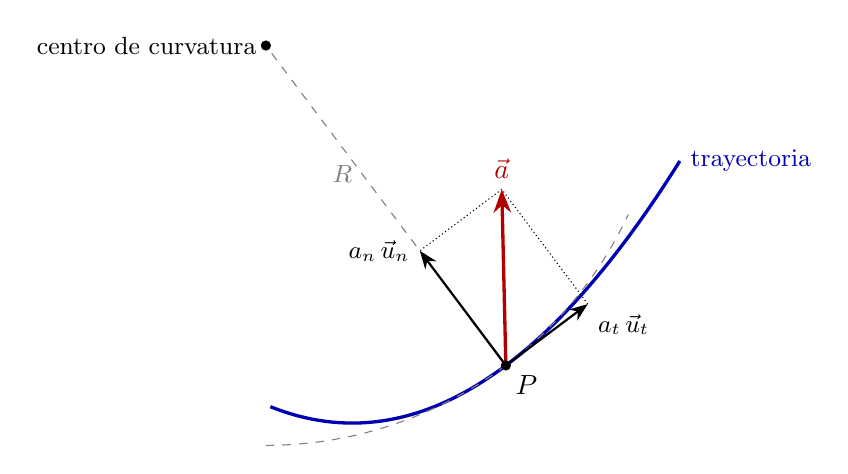
\begin{tikzpicture}[>=Stealth,scale=1.3]
  \draw[very thick,blue!70!black,domain=-0.8:3.2,samples=60] plot (\x,{0.25*\x*\x}) node[right]{\small trayectoria};
  \coordinate (P) at (1.5,0.5625);
  \coordinate (C) at (-0.844,3.6875);
  \draw[dashed,gray] ($(C)+(-90:3.906)$) arc[start angle=-90,end angle=-25,radius=3.906];
  \draw[dashed,gray] (P)--(C) node[pos=0.6,left]{\small $R$};
  \fill (C) circle (0.05) node[left]{\small centro de curvatura};
  % componentes y aceleración: a = 1.0 u_t + 1.4 u_n
  \coordinate (At) at ($(P)+1.0*(0.8,0.6)$);
  \coordinate (An) at ($(P)+1.4*(-0.6,0.8)$);
  \coordinate (A)  at ($(P)+1.0*(0.8,0.6)+1.4*(-0.6,0.8)$);
  \draw[densely dotted] (At)--(A)--(An);
  \draw[->,thick] (P)--(At) node[below right]{\small $a_t\,\vec u_t$};
  \draw[->,thick] (P)--(An) node[left]{\small $a_n\,\vec u_n$};
  \draw[->,very thick,red!70!black] (P)--(A) node[above]{$\vec a$};
  \fill (P) circle (0.05) node[below right]{$P$};
\end{tikzpicture}
\end{center}

\begin{itemize}[itemsep=1pt]
  \item $a_t$ cambia el \emph{módulo} de la velocidad (acelera o frena).
  \item $a_n$ cambia la \emph{dirección} de la velocidad (hace girar). Aunque la rapidez sea constante, si la trayectoria se curva hay aceleración.
\end{itemize}
\begin{tabular}{@{}ll@{}}
MRU: $a_t=0$, $a_n=0$ & MRUA: $a_t\neq0$, $a_n=0$\\
MCU: $a_t=0$, $a_n=\frac{v^2}{R}$ constante & MCUA: $a_t\neq0$ constante, $a_n\neq0$
\end{tabular}

\begin{clave}[title={¿De dónde sale $a_n=v^2/R$?}]
Se ve fácil en un \textbf{movimiento circular uniforme} de radio $R$ y velocidad angular $\omega$ (constante), derivando la posición:
\begin{align*}
\vec r(t)&=R\cos(\omega t)\,\ii+R\sin(\omega t)\,\jj\\
\vec v(t)=\vec r\,'(t)&=-R\omega\sin(\omega t)\,\ii+R\omega\cos(\omega t)\,\jj\qquad\Rightarrow\quad v=|\vec v|=R\omega\\
\vec a(t)=\vec v\,'(t)&=-R\omega^2\cos(\omega t)\,\ii-R\omega^2\sin(\omega t)\,\jj=-\omega^2\,\vec r(t)
\end{align*}
\begin{itemize}[itemsep=1pt]
  \item $\vec a=-\omega^2\vec r$: la aceleración apunta \textbf{hacia el centro} (sentido contrario a $\vec r$). Es puramente normal: $a_t=0$ porque la rapidez $v=R\omega$ no cambia.
  \item Su módulo: $a_n=\omega^2R=\left(\dfrac vR\right)^2R=\dfrac{v^2}{R}$.
\end{itemize}
Idea intuitiva: aunque la rapidez sea siempre la misma, el vector $\vec v$ va girando para seguir la circunferencia, y ese cambio de dirección es una aceleración. Cuanto más rápido se va ($v$ grande) o más cerrada es la curva ($R$ pequeño), mayor es. En una trayectoria cualquiera, en cada punto se aproxima la curva por una circunferencia de radio $R$ (el radio de curvatura) y la fórmula es la misma.
\end{clave}

\begin{ejemplo}[title={Ejemplo (continuación): en $t=1$ s}]
$\vec v=2\ii+2\jj$ ($v=2\sqrt2$ m/s), $\vec a=2\jj$ ($a=2$ m/s$^2$). La tangencial es la proyección de $\vec a$ sobre $\vec v$:
$a_t=\frac{\vec a\cdot\vec v}{v}=\frac{4}{2\sqrt2}=\sqrt2=1{,}41$ m/s$^2$; \ $a_n=\sqrt{a^2-a_t^2}=\sqrt{4-2}=1{,}41$ m/s$^2$; radio de curvatura $R=\frac{v^2}{a_n}=\frac{8}{1{,}41}=5{,}66$ m.
\end{ejemplo}

\textbf{Magnitudes angulares} (movimiento circular de radio $R$): ángulo $\varphi=\frac sR$ (rad), velocidad angular $\omega=\frac vR$ (rad/s), aceleración angular $\alpha=\frac{a_t}{R}$ (rad/s$^2$). En el MCU: $v=\omega R$, $T=\frac{2\pi}{\omega}=\frac{2\pi R}{v}$, $a_n=\frac{v^2}{R}=\omega^2R$.

\subsection{Tiro horizontal}
Es la superposición de un MRU horizontal y una caída libre vertical:
$x=v_0t$, \ $v_x=v_0$; \quad $y=h-\tfrac12gt^2$, \ $v_y=-gt$.
\begin{ejemplo}
Se lanza horizontalmente con $v_0=15$ m/s y tarda 3 s en llegar al suelo.
Altura: $h=\frac12gt^2=\frac12\cdot9{,}8\cdot9=44{,}1$ m. \
Velocidad al llegar: $v_x=15$, $v_y=9{,}8\cdot3=29{,}4$ m/s $\Rightarrow v=\sqrt{15^2+29{,}4^2}=33{,}0$ m/s.
\end{ejemplo}

%=====================================================================
\section{Dinámica}
%=====================================================================
\subsection{Leyes de Newton (repaso)}
Válidas para cuerpos macroscópicos con $v\ll c$ (velocidad de la luz).
\begin{enumerate}[itemsep=2pt]
  \item \textbf{Inercia}: si la fuerza neta es nula, el cuerpo sigue en reposo o con MRU.
  \item \textbf{Fundamental}: $\sum\vec F=m\,\vec a$. La masa inercial es la constante $\frac{F_1}{a_1}=\frac{F_2}{a_2}=m$.
  \item \textbf{Acción y reacción}: si A ejerce $\vec F$ sobre B, B ejerce $-\vec F$ sobre A.
\end{enumerate}

\subsection{Momento lineal (cantidad de movimiento) e impulso}
\[
\vec p=m\,\vec v\quad(\mathrm{kg\cdot m/s}),\qquad \vec I=\vec F\,\Delta t=\Delta\vec p=\vec p_f-\vec p_0\quad(\mathrm{N\cdot s}).
\]
La segunda ley, en su forma general, es $\vec F=\dfrac{d\vec p}{dt}$. El impulso dice que una fuerza actuando durante un tiempo cambia el momento lineal.

\begin{clave}[title={Interpretación del momento lineal y del impulso}]
\begin{itemize}[itemsep=2pt]
  \item $\vec p$ mide \textbf{la ``cantidad de movimiento'' que lleva un cuerpo}: cuánto cuesta pararlo (o cuánto movimiento puede transmitir en un choque). Crece con la masa y con la velocidad, y tiene la dirección y sentido de $\vec v$. Un camión a 10 km/h y una bala a 1000 km/h pueden tener el mismo $\vec p$.
  \item $\vec p$ \textbf{no es una fuerza}, ni la capacidad de ``hacer'' una fuerza concreta. La fuerza que aparece al parar el cuerpo depende de \emph{cuánto tiempo} dure la frenada: $F=\dfrac{\Delta p}{\Delta t}$. El mismo $\Delta p$ en poco tiempo da una fuerza enorme (chocar contra una pared); en más tiempo, una fuerza pequeña (airbag, colchoneta, flexionar las piernas al caer).
  \item \textbf{El impulso es una fuerza actuando durante un tiempo}: $\vec I=\vec F\,\Delta t$. Es la \emph{causa}, y $\Delta\vec p$ (el cambio de momento lineal) es el \emph{efecto}. El teorema dice que son iguales: $\vec I=\Delta\vec p$.
  \item Solo cambia $\vec p$ si la \textbf{fuerza neta} es distinta de cero. Si las fuerzas se compensan (por ejemplo, peso y normal), $\vec p$ no cambia. Y el cambio va en la dirección de la fuerza, que no tiene por qué ser la de $\vec v$: una fuerza perpendicular a $\vec v$ cambia la dirección del movimiento.
\end{itemize}
\end{clave}

\textbf{Principio de conservación}: si $\sum\vec F_{\text{ext}}=\vec 0$, entonces $\vec p$ total se conserva: $\vec p_0=\vec p_f$. Se aplica en choques, explosiones, sistemas aislados, superficies sin rozamiento (hielo).

\begin{ejemplo}[title={Ejemplos}]
\textbf{a)} Un coche de 1000 kg pasa de 0 a 108 km/h $=30$ m/s en 10 s: $\Delta p=1000\cdot30=30\,000$ kg·m/s; \ $F=\frac{\Delta p}{\Delta t}=3000$ N.

\textbf{b)} Una patinadora (60 kg) y un niño (30 kg), en reposo sobre hielo, se empujan; ella sale a 0,4 m/s. Como $\vec p$ total era 0:
$0=60\cdot0{,}4+30\,v_n\Rightarrow v_n=-0{,}8$ m/s (sentido contrario, y el doble de rápido porque tiene la mitad de masa).
\end{ejemplo}

\subsection{Momento angular}\label{sec:L}
\[
\boxed{\ \vec L=\vec r\times\vec p=\vec r\times m\vec v\ }\qquad [L]=\mathrm{kg\cdot\frac{m^2}{s}}
\]
\begin{itemize}[itemsep=2pt]
  \item \textbf{Módulo}: $|\vec L|=r\,m\,v\sin\alpha=m\,v\,d$ \ ($d$: distancia de $O$ a la recta por la que se mueve la partícula).
  \item \textbf{Dirección}: perpendicular al plano formado por $\vec r$ y $\vec v$ (el plano del movimiento).
  \item \textbf{Sentido}: regla de la mano derecha (girando de $\vec r$ hacia $\vec v$).
  \item Siempre se calcula \textbf{respecto a un punto} $O$. Si cambia $O$, cambia $\vec r$ y cambia $\vec L$.
\end{itemize}

\begin{clave}[title={Interpretación del momento angular (en paralelo con el momento lineal)}]
\begin{itemize}[itemsep=2pt]
  \item $\vec L$ mide \textbf{la ``cantidad de giro'' que lleva un cuerpo alrededor de un punto $O$}: cuánto cuesta frenar ese giro. Crece con la masa, con la velocidad y con la distancia $d$ (el brazo): $|\vec L|=m\,v\,d$. Su dirección es la del eje de giro (perpendicular al plano del movimiento) y su sentido, el de la mano derecha.
  \item Depende del punto $O$ elegido. Una partícula que va en línea recta también tiene momento angular respecto a $O$, salvo que su recta pase por $O$ (entonces $d=0$).
\end{itemize}
\begin{center}
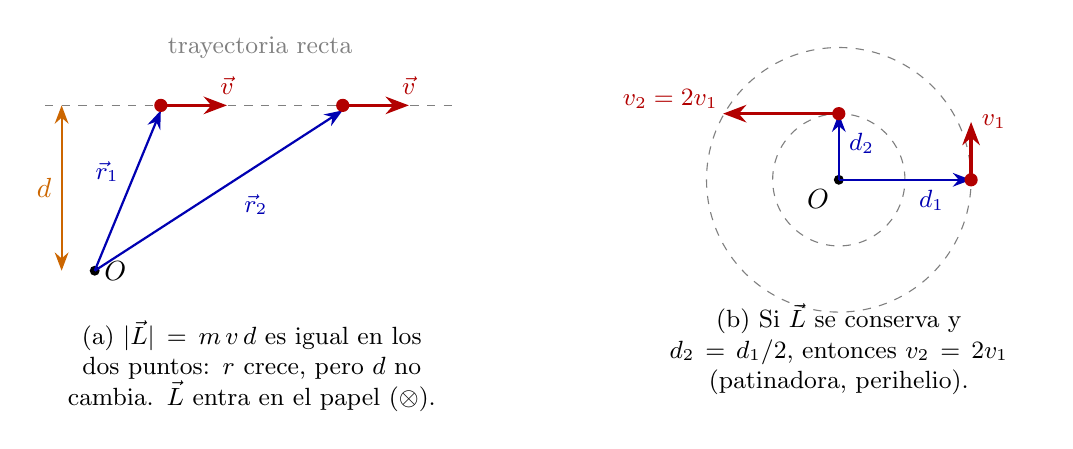
\begin{tikzpicture}[>=Stealth,scale=1.05]
  % (a) partícula en línea recta
  \begin{scope}
    \draw[dashed,gray] (-0.6,2)--(4.4,2);
    \node[gray,font=\small,anchor=south] at (2.0,2.45) {trayectoria recta};
    \fill (0,0) circle (0.06) node[right]{$O$};
    \foreach \x in {0.8, 3.0}{
      \draw[->,thick,blue!70!black] (0,0)--(\x,1.94);
      \fill[red!70!black] (\x,2) circle (0.08);
      \draw[->,very thick,red!70!black] (\x,2)--(\x+0.8,2) node[above,font=\small]{$\vec v$};
    }
    \node[blue!70!black,font=\small] at (0.15,1.2) {$\vec r_1$};
    \node[blue!70!black,font=\small] at (1.95,0.8) {$\vec r_2$};
    \draw[<->,orange!80!black,thick] (-0.4,0)--(-0.4,2) node[midway,left]{$d$};
    \node[align=center,font=\small,text width=5.2cm] at (1.9,-1.15) {(a) $|\vec L|=m\,v\,d$ es igual en los dos puntos: $r$ crece, pero $d$ no cambia. $\vec L$ entra en el papel ($\otimes$).};
  \end{scope}
  % (b) conservación: menor distancia, mayor velocidad
  \begin{scope}[xshift=9cm,yshift=1.1cm]
    \draw[gray,dashed] (0,0) circle (1.6);
    \draw[gray,dashed] (0,0) circle (0.8);
    \fill (0,0) circle (0.06) node[below left]{$O$};
    \draw[->,thick,blue!70!black] (0,0)--(1.6,0) node[pos=0.7,below,font=\small]{$d_1$};
    \draw[->,thick,blue!70!black] (0,0)--(0,0.8) node[pos=0.55,right,font=\small]{$d_2$};
    \fill[red!70!black] (1.6,0) circle (0.08);
    \fill[red!70!black] (0,0.8) circle (0.08);
    \draw[->,very thick,red!70!black] (1.6,0)--(1.6,0.7) node[right,font=\small]{$v_1$};
    \draw[->,very thick,red!70!black] (0,0.8)--(-1.4,0.8) node[above left=-2pt,font=\small]{$v_2=2v_1$};
    \node[align=center,font=\small,text width=5cm] at (0,-2.05) {(b) Si $\vec L$ se conserva y $d_2=d_1/2$, entonces $v_2=2v_1$ (patinadora, perihelio).};
  \end{scope}
\end{tikzpicture}
\end{center}
\begin{itemize}[itemsep=2pt]
  \item $\vec L$ \textbf{no es un momento de fuerza}. Igual que $\vec p$ no es una fuerza, $\vec L$ no es lo que ``hace girar'': es el giro que ya lleva el cuerpo.
  \item \textbf{El momento de una fuerza actuando durante un tiempo cambia el momento angular}: $\Delta\vec L=\vec M\,\Delta t$ (si $\vec M$ es constante). $\vec M$ es la \emph{causa} y $\Delta\vec L$ el \emph{efecto}, igual que $\vec I=\vec F\,\Delta t=\Delta\vec p$. Por eso con la llave larga (más momento) la tuerca gana velocidad de giro más deprisa.
  \item Solo cambia $\vec L$ si el \textbf{momento neto} es distinto de cero. Puede haber fuerza y momento nulo: si la fuerza apunta siempre hacia $O$ (fuerza central), su brazo es cero y $\vec L$ se conserva. Es el caso de la gravedad y los planetas.
  \item Consecuencia de la conservación: si $\vec L$ es constante y la distancia disminuye, la velocidad aumenta ($m\,v\,d$ = constante). La patinadora que recoge los brazos gira más rápido; el planeta va más rápido en el perihelio.
\end{itemize}
\end{clave}

\paragraph{Teorema del momento angular.} Derivando $\vec L=\vec r\times m\vec v$ con la regla del producto:
\[
\frac{d\vec L}{dt}=\underbrace{\vec r\,'\times m\vec v}_{\vec v\times m\vec v=\vec 0}+\vec r\times m\,\vec v\,'=\vec r\times m\vec a=\vec r\times\vec F=\vec M .
\]
El primer término es nulo porque $\vec v$ es paralelo a sí mismo. Resultado: \textbf{la derivada del momento angular es el momento de la fuerza}, $\dfrac{d\vec L}{dt}=\vec M$ (el análogo de $\vec F=\frac{d\vec p}{dt}$).

\paragraph{Conservación del momento angular.} $\vec L$ es constante $\iff\vec M=\vec r\times\vec F=\vec 0$, lo que ocurre si:
\begin{enumerate}[itemsep=1pt]
  \item $\vec r=\vec 0$ (trivial), o
  \item $\vec F=\vec 0$ (partícula libre, MRU), o
  \item $\vec r\parallel\vec F$: la fuerza apunta siempre hacia (o desde) el punto $O$. Es una \textbf{fuerza central}. \textbf{La gravedad es una fuerza central}: este caso es el importante.
\end{enumerate}

\begin{ejemplo}[title={Ejemplo: momento lineal y angular en $t=1$ s}]
\textbf{Datos:} partícula de 2 kg con $\vec r(t)=4t\,\ii+t^2\,\jj$ (m).
\begin{enumerate}[itemsep=3pt]
  \item Velocidad: $\vec v(t)=4\ii+2t\,\jj$. En $t=1$: $\vec r=4\ii+\jj$, \ $\vec v=4\ii+2\jj$, \ $\vec p=m\vec v=8\ii+4\jj$ kg·m/s.
  \item Momento angular:
  \[\vec L=\vec r\times\vec p=\begin{vmatrix}\ii&\jj&\kk\\4&1&0\\8&4&0\end{vmatrix}=\kk\,(4\cdot4-1\cdot8)=8\,\kk\ \ \mathrm{kg\,m^2/s}.\]
  \item \textbf{Comprobación del teorema.} En general $\vec p=8\ii+4t\,\jj$ y $\vec L(t)=\kk\,(4t\cdot4t-t^2\cdot8)=8t^2\,\kk$, que \emph{no} es constante. ¿Por qué? Porque hay fuerza: $\vec a=2\jj$, \ $\vec F=m\vec a=4\jj$ N, y su momento es $\vec M=\vec r\times\vec F=\kk\,(4t\cdot4-0)=16t\,\kk$, que coincide con $\frac{d\vec L}{dt}=16t\,\kk$. \checkmark
\end{enumerate}
\end{ejemplo}

\begin{ejemplo}[title={Ejemplo: respecto a un punto distinto del origen}]
\textbf{Datos:} $m=500$ g $=0{,}5$ kg; \ $\vec r(t)=t^2\,\ii+\jj+2\kk$ (m).\\
\textbf{Se pide:} a) el momento angular $\vec L_P(t)$ y b) el momento de la fuerza $\vec M_P$, ambos respecto al punto $P(0,3,2)$.

\begin{enumerate}[itemsep=4pt]
  \item \textbf{Vector de posición respecto a $P$} (no respecto al origen): se resta la posición de $P$,
  \[\vec r_P=\vec r-\overrightarrow{OP}=(t^2,\,1,\,2)-(0,\,3,\,2)=(t^2,\,-2,\,0)\ \text{m}.\]
  \item \textbf{Velocidad y momento lineal}, derivando $\vec r(t)$:
  \[\vec v=\vec r\,'(t)=(2t,\,0,\,0)\ \text{m/s},\qquad \vec p=m\vec v=(t,\,0,\,0)\ \text{kg·m/s}.\]
  \item \textbf{a) Momento angular}:
  \[\vec L_P=\vec r_P\times\vec p=\begin{vmatrix}\ii&\jj&\kk\\t^2&-2&0\\t&0&0\end{vmatrix}=\kk\,\big(t^2\cdot0-(-2)\cdot t\big)=2t\,\kk\ \ \text{kg·m}^2\text{/s}.\]
  Crece con el tiempo: no se conserva, porque hay una fuerza con momento respecto a $P$.
  \item \textbf{Aceleración y fuerza}, derivando $\vec v(t)$:
  \[\vec a=\vec v\,'(t)=(2,\,0,\,0)\ \text{m/s}^2,\qquad \vec F=m\vec a=(1,\,0,\,0)\ \text{N}.\]
  \item \textbf{b) Momento de la fuerza}:
  \[\vec M_P=\vec r_P\times\vec F=\begin{vmatrix}\ii&\jj&\kk\\t^2&-2&0\\1&0&0\end{vmatrix}=\kk\,\big(t^2\cdot0-(-2)\cdot1\big)=2\,\kk\ \ \text{N·m}.\]
  \item \textbf{Comprobación del teorema}: $\dfrac{d\vec L_P}{dt}=\dfrac{d}{dt}(2t\,\kk)=2\,\kk=\vec M_P$. \checkmark
\end{enumerate}
\end{ejemplo}

\subsection*{Resumen: traslación y rotación en paralelo}
Cada magnitud de la traslación tiene su ``gemela'' en la rotación, que se obtiene haciendo el producto vectorial con $\vec r$ (siempre respecto a un punto $O$):
\begin{center}
\renewcommand{\arraystretch}{1.7}
\begin{tabular}{|>{\raggedright\arraybackslash}p{3.3cm}|>{\raggedright\arraybackslash}p{5.3cm}|>{\raggedright\arraybackslash}p{5.8cm}|}
\hline
 & \textbf{Traslación} & \textbf{Rotación (respecto a $O$)}\\ \hline
Lo que lleva el cuerpo & $\vec p=m\vec v$\newline \textbf{momento lineal} o \textbf{cantidad de movimiento} (kg·m/s) & $\vec L=\vec r\times m\vec v=\vec r\times\vec p$\newline \textbf{momento angular} (kg·m$^2$/s)\\ \hline
Lo que lo cambia & $\vec F$\newline \textbf{fuerza} (N) & $\vec M=\vec r\times\vec F$\newline \textbf{momento de la fuerza} (N·m)\\ \hline
Ley fundamental & $\vec F=\dfrac{d\vec p}{dt}$ & $\vec M=\dfrac{d\vec L}{dt}$\\ \hline
Efecto durante un tiempo & $\vec F\,\Delta t=\Delta\vec p$\newline (impulso) & $\vec M\,\Delta t=\Delta\vec L$\\ \hline
Se conserva si & $\sum\vec F=\vec 0$\newline (sistema aislado, choques) & $\sum\vec M=\vec 0$\newline (p.\,ej. fuerza central: gravedad)\\ \hline
Módulo & $p=m\,v$ & $L=m\,v\,d=r\,m\,v\sin\alpha$ \quad ($d$: brazo)\\ \hline
\end{tabular}
\end{center}

%=====================================================================
\section{Interacción gravitatoria}
%=====================================================================
\subsection{Leyes de Kepler}
Kepler (1609--1619) las obtuvo \emph{empíricamente}, a partir de las observaciones de Tycho Brahe. Newton las explicó después con su ley de gravitación.

\begin{center}
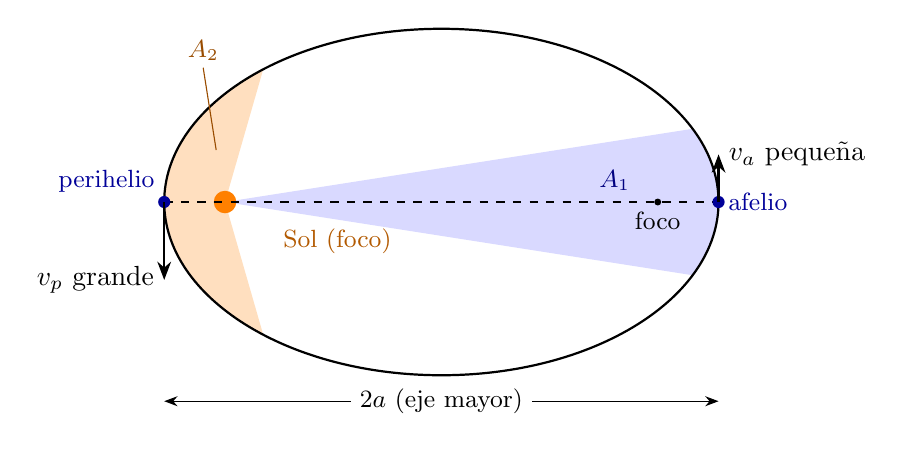
\begin{tikzpicture}[scale=1.1,>=Stealth]
  \def\a{3.2}\def\b{2}
  \pgfmathsetmacro{\c}{sqrt(\a*\a-\b*\b)}
  \fill[blue!15] (-\c,0)--plot[domain=-25:25,samples=30]({\a*cos(\x)},{\b*sin(\x)})--cycle;
  \fill[orange!25] (-\c,0)--plot[domain=130:230,samples=40]({\a*cos(\x)},{\b*sin(\x)})--cycle;
  \draw[thick] (0,0) ellipse ({\a} and {\b});
  \fill[orange] (-\c,0) circle (0.13); \node[orange!70!black] at (-1.2,-0.45) {\small Sol (foco)};
  \fill (\c,0) circle (0.04) node[below]{\small foco};
  \draw[dashed] (-\a,0)--(\a,0);
  \fill[blue!60!black] (-\a,0) circle (0.07) node[above left]{\small perihelio};
  \fill[blue!60!black] (\a,0) circle (0.07) node[right]{\small afelio};
  \draw[->,thick] (-\a,0)--(-\a,-0.9) node[left]{$v_p$ grande};
  \draw[->,thick] (\a,0)--(\a,0.55) node[right]{$v_a$ pequeña};
  \draw[<->] (-\a,-2.3)--(\a,-2.3) node[midway,fill=white]{\small $2a$ (eje mayor)};
  \node[blue!50!black] at (2.0,0.25) {\small $A_1$};
  \node[orange!60!black] at (-2.75,1.75) {\small $A_2$}; \draw[orange!60!black] (-2.75,1.55)--(-2.6,0.6);
\end{tikzpicture}
\end{center}

\begin{enumerate}[itemsep=4pt]
  \item \textbf{Ley de las órbitas}: los planetas describen \emph{órbitas elípticas} con el Sol en uno de los focos. \textbf{Perihelio}: punto más cercano al Sol; \textbf{afelio}: el más lejano. (Las órbitas reales son elipses casi circulares; por eso en los problemas se aproximan por circunferencias.)
  \item \textbf{Ley de las áreas}: el radio vector que une el Sol con el planeta barre \emph{áreas iguales en tiempos iguales}: $\frac{\Delta A}{\Delta t}=$ constante. En la figura, si $A_1=A_2$ se recorren en el mismo tiempo. Consecuencia: el planeta va \emph{más rápido cerca del Sol} y más lento lejos.
  \item \textbf{Ley de los periodos}: los cuadrados de los periodos son proporcionales a los cubos de los semiejes mayores (o del radio, en órbitas circulares):
  \[ T^2=k\,r^3\quad\Longleftrightarrow\quad\frac{T_1^2}{r_1^3}=\frac{T_2^2}{r_2^3}. \]
  La constante $k$ es la \emph{misma para todos los cuerpos que giran alrededor del mismo astro} (depende solo de la masa central).
\end{enumerate}

\subsection{Justificación de la 2.ª ley: conservación del momento angular}\label{sec:areolar}
\begin{enumerate}[itemsep=3pt]
  \item La fuerza gravitatoria del Sol sobre el planeta apunta siempre hacia el Sol: es \textbf{central}. Tomando el Sol como origen, $\vec r\parallel\vec F$.
  \item Por tanto $\vec M=\vec r\times\vec F=\vec 0\Rightarrow\vec L=\vec r\times m\vec v$ es \textbf{constante}.
  \item Que la \emph{dirección} de $\vec L$ sea constante significa que $\vec r$ y $\vec v$ están siempre en el mismo plano: \textbf{la órbita es plana}.
  \item Que el \emph{módulo} sea constante da la ley de las áreas. En un tiempo $dt$, el radio vector barre un triángulo de lados $\vec r$ y $\vec v\,dt$, cuya área es $dA=\frac12|\vec r\times\vec v\,dt|$. Por tanto
  \[ \boxed{\ v_{\text{areolar}}=\frac{dA}{dt}=\frac12|\vec r\times\vec v|=\frac{L}{2m}=\text{constante}\ }\quad(\mathrm{m^2/s}). \]
\end{enumerate}

\textbf{Perihelio y afelio.} En esos dos puntos $\vec r\perp\vec v$ ($\sin\alpha=1$), así que $L=m\,r\,v$ y, al conservarse,
\[ m\,r_p\,v_p=m\,r_a\,v_a\ \Longrightarrow\ \boxed{\ r_p\,v_p=r_a\,v_a\ }\qquad(r_p<r_a\Rightarrow v_p>v_a). \]

\begin{ejemplo}[title={Ejemplo: la Tierra}]
En el perihelio la Tierra está a $1{,}471\cdot10^{11}$ m del Sol y va a 30,29 km/s. En el afelio está a $1{,}521\cdot10^{11}$ m:
$v_a=\frac{r_p\,v_p}{r_a}=\frac{1{,}471}{1{,}521}\cdot30{,}29=29{,}29$ km/s.
\end{ejemplo}

\begin{ojo}
La velocidad orbital solo es constante si la órbita es circular ($r$ constante). En una órbita elíptica varía: máxima en el perihelio, mínima en el afelio. Lo que siempre se conserva es $L$ (y la velocidad areolar).
\end{ojo}

\subsection{Ley de gravitación universal (Newton)}
\emph{Dos cuerpos cualesquiera del universo se atraen con una fuerza directamente proporcional al producto de sus masas e inversamente proporcional al cuadrado de la distancia entre sus centros:}
\[
\boxed{\ F=G\,\frac{M\,m}{r^2}\ }\qquad G=6{,}67\cdot10^{-11}\ \mathrm{N\,m^2/kg^2}.
\]
En forma vectorial, la fuerza que $M$ ejerce sobre $m$ es $\vec F=-G\dfrac{Mm}{r^2}\,\ur$, donde $\ur$ es el vector unitario que va de $M$ hacia $m$; el signo menos indica que es \emph{atractiva} (apunta hacia $M$).
\begin{itemize}[itemsep=2pt]
  \item Es una fuerza central y siempre atractiva. Cumple acción y reacción: $m$ atrae a $M$ con la misma fuerza.
  \item $G$ es muy pequeña: la gravedad solo es apreciable si alguna de las masas es enorme.
  \item Cerca de la Tierra, a una altura $h$: $F=G\frac{M_T\,m}{(R_T+h)^2}$. ¡La distancia es al \emph{centro} de la Tierra!
\end{itemize}

\begin{ejemplo}[title={Ejemplo: fuerza Tierra--Luna}]
$M_T=5{,}97\cdot10^{24}$ kg, $M_L=7{,}35\cdot10^{22}$ kg, $d=3{,}84\cdot10^8$ m:
$F=6{,}67\cdot10^{-11}\cdot\frac{5{,}97\cdot10^{24}\cdot7{,}35\cdot10^{22}}{(3{,}84\cdot10^8)^2}=1{,}98\cdot10^{20}$ N.
(Un problema típico hace el camino inverso: con $F$ dada, se despeja $d=\sqrt{GM_TM_L/F}$.)
\end{ejemplo}

\paragraph{Peso y la relación $G M_T=g_0R_T^2$.} En la superficie, la fuerza gravitatoria es el peso: $G\frac{M_T\,m}{R_T^2}=m\,g_0$, de donde
\[
\boxed{\ G\,M_T=g_0\,R_T^2\ }\qquad(g_0=9{,}8\ \mathrm{m/s^2}).
\]
Este truco permite resolver problemas \emph{sin conocer $G$ ni $M_T$}, solo con $g_0$ y $R_T$. Aparece mucho.

\subsection{Deducción de la 3.ª ley de Kepler (aprender todo el proceso)}
Suponemos una \textbf{órbita circular} de radio $r$ de un cuerpo de masa $m$ alrededor de otro de masa $M$.

\begin{minipage}{0.62\textwidth}
\textbf{Paso 1.} La fuerza gravitatoria es la que obliga a girar, es decir, hace de \textbf{fuerza centrípeta}:
\[
F_g=F_c\quad\Longrightarrow\quad G\frac{M\,m}{r^2}=m\frac{v^2}{r}.
\]
\begin{clave}[title={¿De dónde sale $F_c=m\,v^2/r$?}]
Es la segunda ley de Newton, $F=m\,a$, aplicada a un movimiento circular uniforme. En ese movimiento la aceleración es solo normal, apunta hacia el centro y vale $a_n=\dfrac{v^2}{r}$ (deducido en el apartado~\ref{sec:intr}). Por tanto, la fuerza neta que hace falta para mantener el giro también apunta hacia el centro y vale
\[F_c=m\,a_n=m\,\frac{v^2}{r}.\]
La \textbf{fuerza centrípeta no es una fuerza nueva}: es el nombre que damos a la fuerza neta dirigida al centro que obliga a girar. Según el caso, ese papel lo hace una fuerza concreta: la tensión de una cuerda (piedra atada que se hace girar), el rozamiento (coche en una curva) o, aquí, \textbf{la gravedad}. Por eso se escribe $F_g=F_c$: la fuerza gravitatoria \emph{es} la fuerza centrípeta.
\end{clave}
\textbf{Paso 2.} Se simplifica $m$ (¡no depende de la masa del satélite!) y una $r$:
\[
\boxed{\ v^2=\frac{G\,M}{r}\ }\quad\Longrightarrow\quad v=\sqrt{\frac{GM}{r}} .
\]
\end{minipage}\hfill
\begin{minipage}{0.33\textwidth}
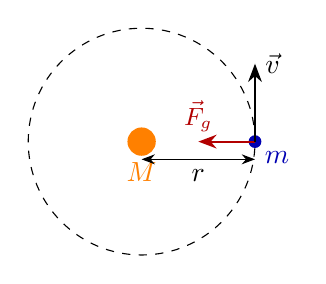
\begin{tikzpicture}[scale=0.9,>=Stealth]
  \draw[dashed] (0,0) circle (1.6);
  \fill[orange] (0,0) circle (0.2) node[below=4pt]{$M$};
  \fill[blue!70!black] (1.6,0) circle (0.09) node[below right]{$m$};
  \draw[->,thick,red!70!black] (1.6,0)--(0.8,0) node[above]{\small $\vec F_g$};
  \draw[->,thick] (1.6,0)--(1.6,1.1) node[right]{$\vec v$};
  \draw[<->] (0,-0.25)--(1.6,-0.25) node[midway,below]{$r$};
\end{tikzpicture}
\end{minipage}

\textbf{Paso 3.} En una vuelta recorre $2\pi r$ en un periodo $T$: $v=\dfrac{2\pi r}{T}$. Igualamos con lo anterior y elevamos al cuadrado:
\[
\frac{4\pi^2r^2}{T^2}=\frac{GM}{r}\quad\Longrightarrow\quad \boxed{\ T^2=\frac{4\pi^2}{G\,M}\,r^3\ }.
\]
\textbf{Conclusión.} Es la 3.ª ley de Kepler con $k=\dfrac{4\pi^2}{GM}$: la constante solo depende de la masa del astro central $M$.

(Alternativa equivalente usando la velocidad angular: $G\frac{Mm}{r^2}=m\,\omega^2r$ con $\omega=\frac{2\pi}{T}$.)

\begin{clave}[title={Para qué sirve}]
\begin{itemize}[itemsep=1pt]
  \item Conocido $T$ y $r$ de un satélite (o planeta), se obtiene la \textbf{masa del astro central}: $M=\dfrac{4\pi^2r^3}{GT^2}$.
  \item Comparando dos cuerpos que orbitan el mismo astro, $\frac{T_1^2}{r_1^3}=\frac{T_2^2}{r_2^3}$, sin necesidad de $G$ ni $M$.
\end{itemize}
\end{clave}

\begin{ejemplo}[title={Ejemplos: masa del Sol y periodo de Júpiter}]
\textbf{Masa del Sol.} La Tierra: $r=1{,}496\cdot10^{11}$ m, $T=1$ año $=3{,}156\cdot10^7$ s:
$M_S=\frac{4\pi^2(1{,}496\cdot10^{11})^3}{6{,}67\cdot10^{-11}\,(3{,}156\cdot10^7)^2}=1{,}99\cdot10^{30}$ kg.

\textbf{Periodo de Júpiter}, sabiendo que está 5,2 veces más lejos del Sol que la Tierra:
$T_J^2=T_T^2\left(\frac{r_J}{r_T}\right)^3=1^2\cdot5{,}2^3=140{,}6\Rightarrow T_J=11{,}86$ años.
\end{ejemplo}

\textbf{Velocidad areolar en órbita circular.} En un periodo se barre el círculo entero: $v_a=\dfrac{\pi r^2}{T}$, que también vale $\frac12 r\,v$. Para la Tierra: $v=\frac{2\pi\cdot1{,}5\cdot10^{11}}{3{,}156\cdot10^7}\approx2{,}99\cdot10^4$ m/s y $v_a=\frac{\pi(1{,}5\cdot10^{11})^2}{3{,}156\cdot10^7}\approx2{,}24\cdot10^{15}$ m$^2$/s.

%=====================================================================
\section{Fuerzas conservativas y energía potencial gravitatoria}
%=====================================================================
\subsection{Trabajo y energía}
\textbf{Trabajo.} Cuando una fuerza constante $\vec F$ actúa sobre un cuerpo que se desplaza $\Delta\vec r$, el trabajo que realiza es
\[
W=\vec F\cdot\Delta\vec r=F\,d\cos\alpha\qquad(\mathrm{J}=\mathrm{N\cdot m}),
\]
donde $d=|\Delta\vec r|$ y $\alpha$ es el ángulo entre la fuerza y el desplazamiento. Es un escalar:
\begin{itemize}[itemsep=1pt]
  \item $\alpha<90^\circ$: $W>0$, la fuerza ayuda al movimiento (aporta energía).
  \item $\alpha=90^\circ$: $W=0$, la fuerza no hace trabajo (p.\,ej. la normal, o la gravedad sobre un satélite en órbita circular).
  \item $\alpha>90^\circ$: $W<0$, la fuerza se opone al movimiento (quita energía; p.\,ej. el rozamiento, $\alpha=180^\circ$).
\end{itemize}
Solo cuenta la componente de la fuerza en la dirección del desplazamiento. Sostener una maleta quieta cansa, pero no hace trabajo: $d=0$.

\textbf{Energía.} Es la capacidad de un cuerpo para realizar trabajo. El trabajo es la forma de \emph{transferir} energía de un cuerpo a otro mediante una fuerza; por eso ambos se miden en julios. En mecánica hay dos formas: la \textbf{energía cinética}, que el cuerpo tiene por moverse, y la \textbf{energía potencial}, que tiene por su posición (ver más abajo).

\textbf{Energía cinética: de dónde sale $E_c=\tfrac12mv^2$.} Empujamos un cuerpo de masa $m$, inicialmente en reposo, con una fuerza constante $F$ a lo largo de una distancia $d$. Es un MRUA con $a=F/m$, y por cinemática $v^2=v_0^2+2ad$, es decir, $a\,d=\dfrac{v^2-v_0^2}{2}$. El trabajo realizado es
\[
W=F\,d=m\,a\,d=m\,\frac{v^2-v_0^2}{2}=\tfrac12mv^2-\tfrac12mv_0^2 .
\]
A la cantidad $\tfrac12mv^2$ se le llama \textbf{energía cinética}. Así:
\begin{itemize}[itemsep=1pt]
  \item $E_c=\tfrac12mv^2$ es el trabajo necesario para llevar el cuerpo desde el reposo hasta la velocidad $v$.
  \item Y, al revés, es el trabajo que puede realizar el cuerpo hasta pararse; o, dicho de otro modo, para detenerlo hay que hacer sobre él un trabajo $-\tfrac12mv^2$ (de frenado).
  \item \textbf{Teorema de la energía cinética}: el trabajo de la fuerza neta es igual a la variación de energía cinética, $W_{\text{total}}=\Delta E_c$. (Vale también para fuerzas variables.)
\end{itemize}

\begin{ojo}
$E_c$ depende de $v^2$: al doble de velocidad, cuatro veces más energía. Un coche a 100 km/h necesita unas cuatro veces más distancia para frenar que a 50 km/h.
\end{ojo}

\subsection{Fuerzas conservativas}
Una fuerza es \textbf{conservativa} si el trabajo que realiza sobre un cuerpo a lo largo de una \emph{trayectoria cerrada} es cero. Equivalentemente, el trabajo para ir de A a B \emph{no depende del camino}, solo de los puntos inicial y final. Son conservativas la gravitatoria, la elástica y la eléctrica; el rozamiento no lo es.

Para estas fuerzas se define una \textbf{energía potencial} $E_p$ tal que
\[
W_{A\to B}=-\Delta E_p=E_{p,A}-E_{p,B}.
\]
Si la fuerza hace trabajo positivo (el cuerpo ``cae'' a favor de la fuerza), la energía potencial disminuye.

\begin{clave}[title={¿Qué hace que una fuerza sea conservativa o no?}]
\begin{itemize}[itemsep=2pt]
  \item \textbf{Conservativa}: la fuerza depende solo de \emph{dónde} está el cuerpo (su posición), no de cómo se mueve. El trabajo que hace al ir de A a B queda ``guardado'' como energía potencial, y se \emph{recupera íntegro} al volver de B a A.
  \item \textbf{No conservativa}: depende del movimiento (velocidad, sentido, camino). El rozamiento se opone siempre al movimiento, así que hace trabajo negativo en la ida \emph{y} en la vuelta: no se recupera nada, y cuanto más largo es el camino, más energía se pierde.
  \item \textbf{¿A dónde va esa energía?} Sí, se convierte en \textbf{calor} (energía térmica: las superficies se calientan), sonido, deformaciones\ldots{} La energía total del universo se sigue conservando; lo que se pierde es energía \emph{mecánica}, porque pasa a una forma desordenada que no se puede volver a convertir en movimiento.
\end{itemize}
\textbf{Ejemplo.} Una caja de 2 kg:
\begin{itemize}[itemsep=1pt]
  \item Se \emph{sube} 1 m y se vuelve a bajar. Gravedad: $-mgh=-19{,}6$ J en la subida y $+19{,}6$ J en la bajada. Total: 0. Es conservativa.
  \item Se \emph{arrastra} 1 m por el suelo y se vuelve ($\mu=0{,}3$). Rozamiento: $-\mu mg\,d=-5{,}9$ J en la ida y otros $-5{,}9$ J en la vuelta. Total: $-11{,}8$ J, que se han convertido en calor. No es conservativa.
\end{itemize}
Cuando hay fuerzas no conservativas, la energía mecánica cambia justo en el trabajo que hacen: $\Delta E_m=W_{\text{no cons}}$ (negativo con rozamiento; puede ser positivo si un motor o una persona aporta energía).
\end{clave}

\textbf{Conservación de la energía mecánica.} Si solo actúan fuerzas conservativas:
\[
E_m=E_c+E_p=\text{constante},\qquad E_c=\tfrac12mv^2,\qquad \Delta E_c=-\Delta E_p .
\]

\subsection{Energía potencial gravitatoria}
\[
\boxed{\ E_p=-G\,\frac{M\,m}{r}\ }\quad(\mathrm J)
\]
\begin{itemize}[itemsep=2pt]
  \item Se toma el \textbf{origen de energía potencial en el infinito}: $E_p(\infty)=0$.
  \item Por eso $E_p$ es \textbf{siempre negativa}: la masa está ``ligada''; hay que aportar energía para alejarla hasta el infinito.
  \item Al acercarse ($r$ menor), $E_p$ se hace más negativa (disminuye); al alejarse, aumenta hacia 0.
\end{itemize}

\begin{clave}[title={¿De dónde sale $E_p=-GMm/r$?}]
La energía potencial se define a partir del trabajo de la fuerza: $W_{A\to B}=E_{p,A}-E_{p,B}$. Elegimos $E_p(\infty)=0$ y calculamos el trabajo que hace la gravedad cuando la masa $m$ se aleja desde una distancia $r$ hasta el infinito:
\[
W_{r\to\infty}=E_p(r)-\underbrace{E_p(\infty)}_{0}=E_p(r).
\]
\begin{itemize}[itemsep=2pt]
  \item La fuerza no es constante (cambia con $1/r^2$), así que no vale $W=F\,d$: hay que sumar los trabajos de tramos pequeños $dr$, es decir, integrar. Al alejarse, la gravedad apunta hacia $M$ y el desplazamiento hacia fuera ($\alpha=180^\circ$), así que cada tramo aporta $-G\frac{Mm}{r^2}\,dr$:
  \[
  W_{r\to\infty}=\int_r^{\infty}-G\frac{Mm}{r^2}\,dr=\left[\,G\frac{Mm}{r}\,\right]_r^{\infty}=0-G\frac{Mm}{r}=-G\frac{Mm}{r}.
  \]
  \item Por tanto $E_p(r)=-G\dfrac{Mm}{r}$. Es negativa porque, al alejar la masa, la gravedad hace trabajo negativo: hay que aportar energía desde fuera para separarla.
  \item \textbf{Comprobación con $mgh$.} Al subir $h$ desde la superficie:
  \[
  \Delta E_p=GM_Tm\left(\frac1{R_T}-\frac1{R_T+h}\right)=GM_Tm\,\frac{h}{R_T(R_T+h)}\ \approx\ \frac{GM_T}{R_T^2}\,m\,h=m\,g_0\,h\quad\text{si } h\ll R_T .
  \]
  La fórmula de cursos anteriores es un caso particular de esta.
\end{itemize}
\textbf{La idea sin integrales: el trabajo es un área.} Si la fuerza fuera constante, $W=F\cdot d$ sería el área de un rectángulo de altura $F$ y base $d$. Como la gravedad cambia con la distancia, se divide el camino en tramos pequeños; en cada uno la fuerza casi no cambia y su trabajo es el área de un rectángulo estrecho. Sumando todos los rectángulos se obtiene el \textbf{área bajo la curva} $F(r)$. Cuanto más estrechos los tramos, mejor se ajustan a la curva; ``integrar'' es justo hacer esa suma con tramos infinitamente estrechos.
\begin{center}
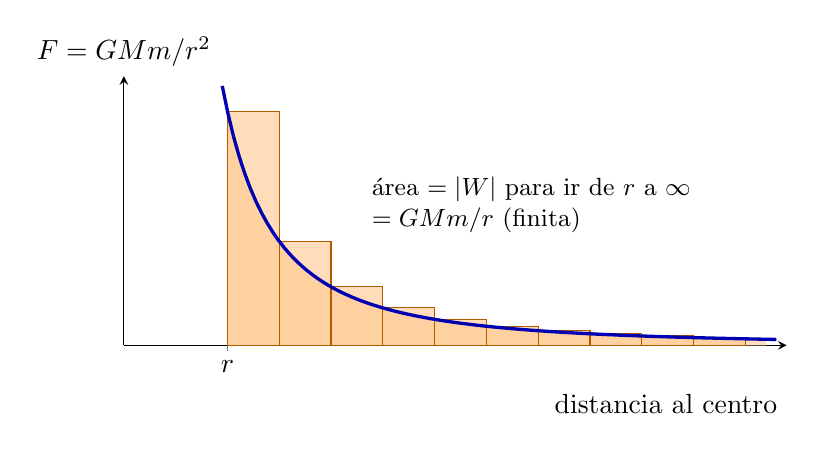
\begin{tikzpicture}
\begin{axis}[width=10cm,height=5cm,axis lines=left,xmin=0,xmax=6.4,ymin=0,ymax=1.15,clip=false,
  xtick={1}, xticklabels={$r$}, ytick=\empty, xlabel={distancia al centro}, ylabel={$F=GMm/r^2$},
  every axis x label/.style={at={(current axis.right of origin)},anchor=north east,yshift=-14pt},
  every axis y label/.style={at={(current axis.above origin)},anchor=south}]
  \addplot[fill=orange!25,draw=none,domain=1:6.2,samples=80] {1/x^2} \closedcycle;
  \foreach \a in {1,1.5,...,5.5}{
    \addplot[draw=orange!70!black,fill=orange!45,fill opacity=0.6] coordinates {(\a,0) (\a,{1/(\a*\a)}) (\a+0.5,{1/(\a*\a)}) (\a+0.5,0)} -- cycle;
  }
  \addplot[very thick,blue!70!black,domain=0.95:6.3,samples=100] {1/x^2};
  \node[anchor=west,font=\small,align=left] at (axis cs:2.3,0.6) {área $=|W|$ para ir de $r$ a $\infty$\\ $=GMm/r$ (finita)};
\end{axis}
\end{tikzpicture}
\end{center}
Aunque el camino hasta el infinito es infinito, la fuerza se hace tan pequeña que el área total es finita y vale $GMm/r$. Con el signo menos (la gravedad tira hacia dentro mientras nos alejamos) queda $E_p=-GMm/r$.
\end{clave}

\begin{center}
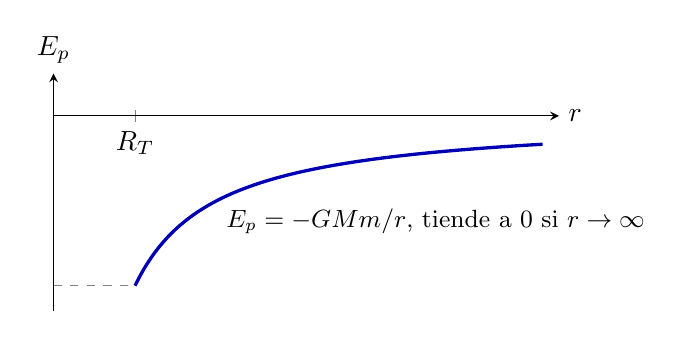
\begin{tikzpicture}
\begin{axis}[width=8cm,height=4.6cm,axis lines=middle,xmin=0,xmax=6.2,ymin=-1.15,ymax=0.25,clip=false,
  xtick={1}, xticklabels={$R_T$}, ytick=\empty, xlabel=$r$, ylabel=$E_p$,
  every axis x label/.style={at={(ticklabel* cs:1)},anchor=west},
  every axis y label/.style={at={(ticklabel* cs:1)},anchor=south}]
  \addplot[very thick,blue!70!black,domain=1:6,samples=100]{-1/x};
  \addplot[dashed,gray,domain=0:1]{-1};
  \node[anchor=west] at (axis cs:2.0,-0.62) {\small $E_p=-GMm/r$, tiende a 0 si $r\to\infty$};
\end{axis}
\end{tikzpicture}
\end{center}

\textbf{Variación al subir una altura $h$ desde la superficie:}
\[
\Delta E_p=E_p(R_T+h)-E_p(R_T)=-G\frac{M_Tm}{R_T+h}+G\frac{M_Tm}{R_T}=G\,M_T\,m\left(\frac1{R_T}-\frac1{R_T+h}\right)>0.
\]
\begin{ojo}[title={Relación con $mgh$}]
La fórmula $E_p=mgh$ de cursos anteriores es una \emph{aproximación} válida solo si $h\ll R_T$ (entonces $g$ es prácticamente constante). Para satélites, órbitas, etc., hay que usar siempre $-GMm/r$.
\end{ojo}

%=====================================================================
\section{Satelización}
%=====================================================================
Satélite de masa $m_s$ en órbita circular de radio $r=R_T+h$ alrededor de la Tierra.

\subsection{Velocidad orbital y periodo}
Igual que en la deducción de Kepler ($F_g=F_c$):
\[
\boxed{\ v_{\text{orb}}=\sqrt{\frac{G\,M_T}{r}}=\sqrt{\frac{g_0R_T^2}{r}}\ }\qquad T=\frac{2\pi r}{v}=2\pi\sqrt{\frac{r^3}{GM_T}} .
\]
Cuanto más lejos, \emph{más despacio} gira y mayor es el periodo. No depende de la masa del satélite.

\subsection{Energía de un satélite en órbita}
\begin{align*}
E_c&=\tfrac12m_sv^2=\tfrac12m_s\frac{GM_T}{r}=\ \ \frac{G\,M_T\,m_s}{2r}\\
E_p&=-\frac{G\,M_T\,m_s}{r}\\
E_{\text{orb}}=E_c+E_p&=\frac{GM_Tm_s}{2r}-\frac{GM_Tm_s}{r}=\boxed{\ -\frac{G\,M_T\,m_s}{2r}\ }
\end{align*}
\begin{clave}[title={Relaciones muy útiles (órbita circular)}]
\[ E_p=-2E_c,\qquad E_{\text{orb}}=-E_c=\tfrac12E_p<0 . \]
La energía total es negativa: el satélite está \emph{ligado} a la Tierra. (Por ejemplo, si $E=-10^{10}$ J, entonces $E_c=10^{10}$ J y $E_p=-2\cdot10^{10}$ J.)
\end{clave}

\subsection{Energía de satelización y velocidad de lanzamiento}
\textbf{Energía de satelización}: energía que hay que dar a un satélite en la superficie para ponerlo en órbita circular de radio $r$. Como la gravedad es conservativa, aplicamos conservación de la energía entre la superficie (donde se lanza con $v_0$) y la órbita:
\[
\underbrace{\tfrac12m_sv_0^2-\frac{GM_Tm_s}{R_T}}_{E\ \text{en la superficie}}=\underbrace{-\frac{GM_Tm_s}{2r}}_{E_{\text{orb}}}
\quad\Longrightarrow\quad
E_{c,\text{sup}}=\tfrac12m_sv_0^2=G\,M_T\,m_s\left(\frac1{R_T}-\frac1{2r}\right).
\]
Despejando, la \textbf{velocidad de lanzamiento}:
\[
\boxed{\ v_0=\sqrt{2\,G\,M_T\left(\frac1{R_T}-\frac1{2r}\right)}\ }
\]
(Se desprecia el rozamiento con el aire y la rotación de la Tierra.)

\textbf{Cambio de órbita} (de radio $r_1$ a $r_2$): el trabajo necesario es la diferencia de energías orbitales,
\[
W=E_{\text{orb},f}-E_{\text{orb},i}=\frac{G\,M_T\,m_s}{2}\left(\frac1{r_1}-\frac1{r_2}\right).
\]
(Pasar a una órbita más alta cuesta energía, aunque luego el satélite vaya más despacio.)

\subsection{Velocidad de escape}
Es la velocidad mínima que hay que comunicar a un cuerpo en la superficie para que \emph{escape} de la atracción terrestre, es decir, llegue al infinito ($E_p=0$) con velocidad nula ($E_c=0$). Por conservación de la energía:
\[
\tfrac12mv_e^2-\frac{GM_Tm}{R_T}=0+0\quad\Longrightarrow\quad\boxed{\ v_e=\sqrt{\frac{2\,G\,M_T}{R_T}}=\sqrt{2g_0R_T}\ }\approx11{,}2\ \mathrm{km/s}.
\]
\begin{ojo}
La velocidad de escape se deduce \textbf{por energía} (energía mecánica total igual a 0), no igualando fuerzas. Tampoco depende de la masa del cuerpo ni de la dirección de lanzamiento.
\end{ojo}

\begin{ejemplo}[title={Ejemplo completo: satélite a 800 km}]
Satélite de 500 kg a $h=800$ km. Datos: $G=6{,}67\cdot10^{-11}$, $M_T=5{,}97\cdot10^{24}$ kg, $R_T=6{,}37\cdot10^6$ m.

$r=R_T+h=7{,}17\cdot10^6$ m; \ $GM_T=3{,}98\cdot10^{14}$ m$^3$/s$^2$.
\begin{enumerate}[itemsep=2pt]
  \item Velocidad orbital: $v=\sqrt{\frac{3{,}98\cdot10^{14}}{7{,}17\cdot10^6}}=7{,}45\cdot10^3$ m/s.
  \item Periodo: $T=\frac{2\pi r}{v}=6045$ s $\approx1{,}68$ h. \ Aceleración centrípeta: $a=\frac{v^2}{r}=7{,}75$ m/s$^2$ (es justo $g$ a esa altura).
  \item Energías: $E_c=\frac{GM_Tm}{2r}=1{,}39\cdot10^{10}$ J; \ $E_p=-2{,}78\cdot10^{10}$ J; \ $E_{\text{orb}}=-1{,}39\cdot10^{10}$ J.
  \item Energía para ponerlo en órbita desde la superficie: $GM_Tm\left(\frac1{R_T}-\frac1{2r}\right)=1{,}74\cdot10^{10}$ J, es decir, velocidad de lanzamiento $v_0=8{,}34$ km/s.
  \item Velocidad de escape (no depende del satélite): $v_e=\sqrt{\frac{2\cdot3{,}98\cdot10^{14}}{6{,}37\cdot10^6}}=11{,}2$ km/s.
\end{enumerate}
\end{ejemplo}

%=====================================================================
\section{Campo gravitatorio}
%=====================================================================
\subsection{Concepto de campo}
En un punto del espacio \textbf{hay campo gravitatorio} si, al colocar en él una partícula con masa (masa de prueba), aparece sobre ella una fuerza gravitatoria. 

\textbf{Definición}: el campo gravitatorio es la \emph{perturbación que un cuerpo produce en el espacio que lo rodea por el hecho de tener masa}. La idea importante es que la masa $M$ ``modifica'' el espacio aunque no haya nada más; cuando ponemos otra masa $m$, el campo actúa sobre ella. Así se separa la \emph{causa} ($M$, que crea el campo) del \emph{efecto} (la fuerza sobre $m$).

\subsection{Intensidad del campo gravitatorio}
Es la fuerza que actúa sobre la unidad de masa colocada en ese punto:
\[
\vec g=\frac{\vec F}{m}\qquad\Longrightarrow\qquad\boxed{\ \vec g=-G\,\frac{M}{r^2}\,\ur\ }\qquad\left(\mathrm{\tfrac Nkg}=\mathrm{\tfrac m{s^2}}\right)
\]
\begin{itemize}[itemsep=2pt]
  \item \textbf{Módulo}: $g=G\dfrac{M}{r^2}$. No depende de la masa de prueba $m$, solo de $M$ y de la distancia.
  \item \textbf{Dirección}: la recta que une $M$ con el punto. $\ur$ es el vector unitario que va \emph{desde $M$ hacia el punto}.
  \item \textbf{Sentido}: hacia $M$ (de ahí el signo menos). El campo gravitatorio siempre apunta hacia la masa que lo crea.
  \item Las unidades N/kg y m/s$^2$ son equivalentes: $\frac{\mathrm N}{\mathrm{kg}}=\frac{\mathrm{kg\cdot m/s^2}}{\mathrm{kg}}=\mathrm{m/s^2}$. Es decir, $\vec g$ es la aceleración que adquiere cualquier cuerpo en ese punto.
\end{itemize}

\textbf{Variación con la altura.} Usando $GM_T=g_0R_T^2$:
\[
g(h)=G\frac{M_T}{(R_T+h)^2}=g_0\left(\frac{R_T}{R_T+h}\right)^2 .
\]
\begin{center}
\begin{tabular}{lcccc}
\toprule
Altura $h$ & $0$ & $400$ km (ISS) & $R_T$ & $2R_T$\\
Distancia al centro $r$ & $R_T$ & $1{,}06\,R_T$ & $2R_T$ & $3R_T$\\
$g$ (m/s$^2$) & $9{,}8$ & $8{,}7$ & $9{,}8/4=2{,}45$ & $9{,}8/9=1{,}09$\\
\bottomrule
\end{tabular}
\end{center}
Si $h\ll R_T$, $g\approx g_0=9{,}8$ m/s$^2$; si $h$ es comparable a $R_T$, ya no.
\begin{ojo}
Error frecuente: confundir la \emph{altura} $h$ con la \emph{distancia al centro} $r=R_T+h$. A una altura $h=R_T$ la distancia al centro es $2R_T$ y $g=g_0/4=2{,}45$ m/s$^2$; a $h=2R_T$ la distancia es $3R_T$ y $g=g_0/9=1{,}09$ m/s$^2$.
\end{ojo}

\subsection{Principio de superposición}
Si hay varias masas, el campo total en un punto $P$ es la \textbf{suma vectorial} de los campos que crea cada una por separado:
\[
\vec g_P=\vec g_1+\vec g_2+\cdots=\sum_{i=1}^n\vec g_i .
\]
\textbf{Procedimiento}:
\begin{enumerate}[itemsep=1pt]
  \item Dibujar en $P$ cada $\vec g_i$, apuntando \emph{desde $P$ hacia la masa $m_i$}.
  \item Calcular cada módulo $g_i=G\frac{m_i}{r_i^2}$ ($r_i$: distancia de $m_i$ a $P$).
  \item Descomponer en componentes $x$ e $y$ (con senos y cosenos si hace falta) y sumar.
  \item Dar el resultado como vector, y si se pide, su módulo.
\end{enumerate}

\begin{ejemplo}[title={Ejemplo: masas alineadas}]
$m_1=2$ kg y $m_2=6$ kg separadas 6 m; $P$ en el punto medio (a 3 m de cada una). $\vec g_1$ apunta hacia $m_1$ ($-\ii$) y $\vec g_2$ hacia $m_2$ ($+\ii$):
$\vec g_P=\left(\frac{Gm_2}{r^2}-\frac{Gm_1}{r^2}\right)\ii=\frac{6{,}67\cdot10^{-11}}{9}(6-2)\,\ii=2{,}96\cdot10^{-11}\,\ii$ N/kg (hacia la masa mayor).
\end{ejemplo}

\begin{ejemplo}[title={Ejemplo: masas en los ejes}]
\begin{minipage}{0.62\textwidth}
$m_1=4$ kg en $(3,0)$ y $m_2=9$ kg en $(0,-3)$ (m). Campo en el origen.
\begin{itemize}[itemsep=1pt]
  \item $g_1=\frac{G\cdot4}{3^2}=2{,}96\cdot10^{-11}$, apunta hacia $+\ii$.
  \item $g_2=\frac{G\cdot9}{3^2}=6{,}67\cdot10^{-11}$, apunta hacia $-\jj$.
\end{itemize}
$\vec g_O=2{,}96\cdot10^{-11}\,\ii-6{,}67\cdot10^{-11}\,\jj$ N/kg;\\
$|\vec g_O|=\sqrt{2{,}96^2+6{,}67^2}\cdot10^{-11}=7{,}30\cdot10^{-11}$ N/kg.
\end{minipage}\hfill
\begin{minipage}{0.33\textwidth}
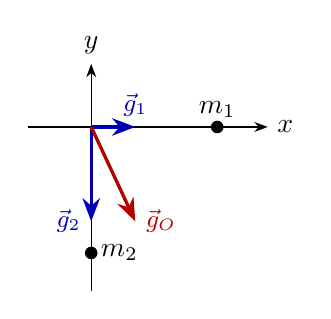
\begin{tikzpicture}[scale=0.8,>=Stealth]
  \draw[->] (-1,0)--(2.8,0) node[right]{$x$};
  \draw[->] (0,-2.6)--(0,1) node[above]{$y$};
  \fill (2,0) circle (0.1) node[above]{$m_1$};
  \fill (0,-2) circle (0.1) node[right]{$m_2$};
  \draw[->,very thick,blue!70!black] (0,0)--(0.7,0) node[above]{\small $\vec g_1$};
  \draw[->,very thick,blue!70!black] (0,0)--(0,-1.5) node[left]{\small $\vec g_2$};
  \draw[->,very thick,red!70!black] (0,0)--(0.7,-1.5) node[right]{\small $\vec g_O$};
\end{tikzpicture}
\end{minipage}
\end{ejemplo}

\newpage
%=====================================================================
\section{Formulario resumen}
%=====================================================================
\subsection*{Variables, unidades y constantes}
\begin{center}\small
\renewcommand{\arraystretch}{1.15}
\begin{tabular}{|>{\centering\arraybackslash}p{2.3cm}|>{\centering\arraybackslash}p{3cm}|>{\raggedright\arraybackslash}p{9.4cm}|}
\hline
\textbf{Notación} & \textbf{Unidades (SI)} & \textbf{Significado}\\ \hline
\multicolumn{3}{|l|}{\textit{Cinemática}}\\ \hline
$\vec r$, $r$ & m & Vector de posición (respecto a un origen $O$) y su módulo (distancia a $O$)\\ \hline
$\Delta\vec r$ & m & Vector desplazamiento entre dos posiciones\\ \hline
$\vec v$, $v$ & m/s & Velocidad y su módulo (rapidez)\\ \hline
$\vec a$ & m/s$^2$ & Aceleración\\ \hline
$a_t$, $a_n$ & m/s$^2$ & Componentes tangencial (cambia la rapidez) y normal (cambia la dirección) de $\vec a$\\ \hline
$R$ & m & Radio de curvatura de la trayectoria (o radio de la circunferencia)\\ \hline
$\omega$ & rad/s & Velocidad angular\\ \hline
$T$ & s & Periodo: tiempo de una vuelta completa\\ \hline
$f$ & Hz $=$ s$^{-1}$ & Frecuencia: vueltas por segundo, $f=1/T$\\ \hline
\multicolumn{3}{|l|}{\textit{Dinámica}}\\ \hline
$m$ & kg & Masa\\ \hline
$\vec F$ & N $=$ kg·m/s$^2$ & Fuerza\\ \hline
$\vec p$ & kg·m/s & Momento lineal o cantidad de movimiento, $m\vec v$\\ \hline
$\vec I$ & N·s & Impulso: fuerza actuando durante un tiempo, $\vec F\Delta t$\\ \hline
$\vec L$ & kg·m$^2$/s & Momento angular respecto a un punto, $\vec r\times m\vec v$\\ \hline
$\vec M$ & N·m & Momento de una fuerza respecto a un punto, $\vec r\times\vec F$\\ \hline
$d$ & m & Brazo: distancia del punto $O$ a la recta de acción del vector\\ \hline
$v_a$ & m$^2$/s & Velocidad areolar: área barrida por el radio vector por segundo\\ \hline
\multicolumn{3}{|l|}{\textit{Energía y gravitación}}\\ \hline
$W$ & J $=$ N·m & Trabajo de una fuerza\\ \hline
$E_c$ & J & Energía cinética, $\tfrac12mv^2$\\ \hline
$E_p$ & J & Energía potencial (gravitatoria: $-GMm/r$, cero en el infinito)\\ \hline
$E_m$ & J & Energía mecánica, $E_c+E_p$\\ \hline
$\vec g$, $g$ & N/kg $=$ m/s$^2$ & Intensidad del campo gravitatorio (fuerza por unidad de masa)\\ \hline
$h$ & m & Altura sobre la superficie (¡no es la distancia al centro, $r=R_T+h$!)\\ \hline
$r_p$, $r_a$ & m & Distancias al Sol en el perihelio y en el afelio\\ \hline
$v_{\text{orb}}$, $v_0$, $v_e$ & m/s & Velocidad orbital, de lanzamiento y de escape\\ \hline
\multicolumn{3}{|l|}{\textit{Constantes}}\\ \hline
$G$ & N·m$^2$/kg$^2$ & Constante de gravitación universal: $6{,}67\cdot10^{-11}$\\ \hline
$g_0$ & m/s$^2$ & Gravedad en la superficie terrestre: $9{,}8$\\ \hline
$M_T$ & kg & Masa de la Tierra: $5{,}97\cdot10^{24}$\\ \hline
$R_T$ & m & Radio de la Tierra: $6{,}37\cdot10^{6}$ (6370 km)\\ \hline
\end{tabular}
\end{center}

\subsection*{Fórmulas}
\begin{center}
\renewcommand{\arraystretch}{1.6}
\begin{tabular}{|p{4.3cm}|p{10.6cm}|}
\hline
Producto escalar & $\vec u\cdot\vec v=|\vec u||\vec v|\cos\alpha=u_xv_x+u_yv_y+u_zv_z$\\ \hline
Producto vectorial & $|\vec u\times\vec v|=|\vec u||\vec v|\sin\alpha$, \ $\perp$ a ambos, mano derecha; determinante\\ \hline
Cinemática & $\vec v=\vec r\,'(t)$, \ $\vec a=\vec v\,'(t)$, \ $a_n=v^2/R$, \ $|\vec a|=\sqrt{a_t^2+a_n^2}$\\ \hline
Momento lineal, impulso & $\vec p=m\vec v$, \ $\vec I=\vec F\Delta t=\Delta\vec p$; \ $\sum\vec F_{\text{ext}}=0\Rightarrow\vec p$ cte\\ \hline
Momento angular & $\vec L=\vec r\times m\vec v$, \ $\frac{d\vec L}{dt}=\vec r\times\vec F$; \ fuerza central $\Rightarrow\vec L$ cte\\ \hline
Kepler & $r_pv_p=r_av_a$; \ $v_a=\frac{dA}{dt}=\frac{L}{2m}$; \ $T^2=\frac{4\pi^2}{GM}r^3$\\ \hline
Gravitación & $F=G\frac{Mm}{r^2}$, \ $G=6{,}67\cdot10^{-11}$ N\,m$^2$/kg$^2$, \ $GM_T=g_0R_T^2$\\ \hline
Energía potencial & $E_p=-G\frac{Mm}{r}$ \ (cero en el infinito); \ $W=-\Delta E_p$\\ \hline
Órbita circular & $v=\sqrt{GM/r}$, \ $T=2\pi r/v$, \ $E_c=\frac{GMm}{2r}$, \ $E_{\text{orb}}=-\frac{GMm}{2r}=-E_c=\frac12E_p$\\ \hline
Lanzamiento y escape & $v_0=\sqrt{2GM\left(\frac1{R}-\frac1{2r}\right)}$, \ $v_e=\sqrt{\frac{2GM}{R}}$\\ \hline
Campo gravitatorio & $\vec g=\frac{\vec F}{m}=-G\frac{M}{r^2}\ur$, \ $g(h)=g_0\left(\frac{R_T}{R_T+h}\right)^2$, \ $\vec g_P=\sum\vec g_i$\\ \hline
\end{tabular}
\end{center}

\newpage
%=====================================================================
\section{Problemas}
%=====================================================================
Para cada tema: dos problemas sencillos ($\star$), dos de nivel medio ($\star\star$) y dos difíciles tipo PAU ($\star\star\star$). Datos, salvo que se indique otra cosa: $G=6{,}67\cdot10^{-11}$ N·m$^2$/kg$^2$, $g_0=9{,}8$ m/s$^2$, $M_T=5{,}97\cdot10^{24}$ kg, $R_T=6{,}37\cdot10^{6}$ m.

\newcommand{\prob}[1]{\item[\textbf{#1}]}

\subsection*{P1. Cálculo vectorial}
\begin{enumerate}[leftmargin=1.4cm,itemsep=5pt]
\prob{1.1 $\star$} Dados $\vec a=3\ii-2\jj+\kk$ y $\vec b=\ii+4\jj-2\kk$, calcula $\vec a+\vec b$, $2\vec a-\vec b$, $|\vec a|$, $\vec a\cdot\vec b$ y el ángulo que forman.
\prob{1.2 $\star$} a) Una fuerza de 50 N forma $120^\circ$ con el eje $X$ positivo. Halla sus componentes. b) Halla el módulo y el ángulo con el eje $X$ del vector $\vec v=(-6,8)$ m/s. ¿En qué cuadrante está?
\prob{1.3 $\star\star$} Dados $\vec a=2\ii+\jj-\kk$ y $\vec b=\ii-\jj+3\kk$: a) calcula $\vec a\times\vec b$; b) comprueba que es perpendicular a ambos; c) halla el área del paralelogramo que forman.
\prob{1.4 $\star\star$} a) Halla $m$ para que $\vec u=(m,2,-1)$ y $\vec v=(3,m,4)$ sean perpendiculares. b) Para ese valor, calcula un vector unitario en la dirección de $\vec v$.
\prob{1.5 $\star\star\star$} Una fuerza $\vec F=2\ii-\jj+3\kk$ (N) está aplicada en el punto $P(1,2,0)$ (m). a) Calcula su momento respecto al origen $O$ y su módulo. b) Calcula su momento respecto a $Q(0,1,1)$. c) ¿A qué distancia de $O$ pasa la recta de acción de la fuerza?
\prob{1.6 $\star\star\star$} Los puntos $A(1,0,0)$, $B(0,2,0)$ y $C(0,0,3)$ forman un triángulo. a) Calcula su área usando el producto vectorial. b) Halla un vector unitario perpendicular al plano del triángulo.
\end{enumerate}

\subsection*{P2. Cinemática}
\begin{enumerate}[leftmargin=1.4cm,itemsep=5pt]
\prob{2.1 $\star$} Una partícula se mueve según $\vec r(t)=2t\,\ii+(5-t^2)\,\jj$ (m). Halla la velocidad y la aceleración en función del tiempo, y sus valores en $t=1$ s.
\prob{2.2 $\star$} Desde una ventana a 45 m de altura se lanza horizontalmente una pelota a 12 m/s. Calcula el tiempo que tarda en llegar al suelo, a qué distancia cae y con qué velocidad llega.
\prob{2.3 $\star\star$} $\vec r(t)=(t^3-3t)\,\ii+2t^2\,\jj$ (m). a) Halla $\vec v(t)$ y $\vec a(t)$. b) ¿En qué instante es nula la componente $x$ de la velocidad? c) Calcula el desplazamiento y la velocidad media entre $t=0$ y $t=2$ s.
\prob{2.4 $\star\star$} Un tiovivo de radio 0,5 m gira a 120 rpm con velocidad angular constante. Calcula $\omega$ en rad/s, el periodo, la velocidad de un punto del borde y su aceleración. ¿Qué tipo de aceleración es?
\prob{2.5 $\star\star\star$} Una partícula se mueve según $\vec r(t)=t\,\ii+t^2\,\jj$ (m). a) Halla la ecuación de la trayectoria. b) En $t=1$ s, calcula las componentes tangencial y normal de la aceleración. c) Calcula el radio de curvatura en ese instante.
\prob{2.6 $\star\star\star$} Se lanza un balón desde el suelo con 20 m/s formando $30^\circ$ con la horizontal. a) Altura máxima y tiempo de vuelo. b) Alcance. c) Velocidad en el punto más alto. d) Radio de curvatura de la trayectoria en ese punto. (Pista: allí la aceleración es toda normal.)
\end{enumerate}

\subsection*{P3. Dinámica: momento lineal y momento angular}
\begin{enumerate}[leftmargin=1.4cm,itemsep=5pt]
\prob{3.1 $\star$} Una pelota de 200 g llega a una pared a 15 m/s y rebota en sentido contrario a 10 m/s. a) Calcula el impulso que recibe. b) Si el contacto dura 0,01 s, ¿qué fuerza media ejerce la pared?
\prob{3.2 $\star$} Una partícula de 3 kg está en $\vec r=2\ii$ (m) y se mueve con $\vec v=4\jj$ (m/s). Calcula su momento lineal y su momento angular respecto al origen. ¿Gira en sentido horario o antihorario?
\prob{3.3 $\star\star$} a) Un rifle de 4 kg dispara una bala de 20 g a 400 m/s. ¿Con qué velocidad retrocede el rifle? b) Si la bala se incrusta en un bloque de madera de 2 kg en reposo sobre una superficie sin rozamiento, ¿a qué velocidad se mueve el conjunto?
\prob{3.4 $\star\star$} Una partícula de 0,5 kg se mueve según $\vec r(t)=t^2\,\ii+2t\,\jj$ (m). Calcula $\vec p(t)$, la fuerza que actúa, $\vec L(t)$ y $\vec M(t)$ respecto al origen, y comprueba que $\frac{d\vec L}{dt}=\vec M$.
\prob{3.5 $\star\star\star$} Una partícula de 2 kg se mueve con velocidad constante $\vec v=4\ii$ m/s por la recta $y=3$ m. a) Calcula su momento angular respecto al origen y comprueba que no depende de su posición. b) Calcula su momento angular respecto a $A(0,3)$ y respecto a $B(5,-1)$. c) Explica por qué en los tres casos es constante.
\prob{3.6 $\star\star\star$} Una bolita de 0,3 kg, atada a una cuerda que pasa por un agujero en el centro de una mesa sin rozamiento, gira con radio 0,8 m a 2 m/s. Se tira de la cuerda desde abajo hasta que el radio es 0,4 m. a) ¿Por qué se conserva el momento angular respecto al agujero? b) Calcula la nueva velocidad. c) Calcula la energía cinética antes y después. ¿De dónde sale la diferencia?
\end{enumerate}

\subsection*{P4. Interacción gravitatoria y leyes de Kepler}
\begin{enumerate}[leftmargin=1.4cm,itemsep=5pt]
\prob{4.1 $\star$} Calcula la fuerza de atracción entre dos esferas de 1000 kg cuyos centros están a 2 m. ¿Por qué no notamos esta fuerza en la vida diaria?
\prob{4.2 $\star$} Marte está 1,52 veces más lejos del Sol que la Tierra. Usando la 3.ª ley de Kepler, calcula su periodo en años terrestres.
\prob{4.3 $\star\star$} Calcula el peso de una persona de 80 kg en la superficie terrestre y a una altura igual al radio terrestre. Usa solo $g_0$ y $R_T$.
\prob{4.4 $\star\star$} La Luna gira alrededor de la Tierra en una órbita aproximadamente circular de radio $3{,}84\cdot10^8$ m con un periodo de 27,3 días. Calcula la masa de la Tierra.
\prob{4.5 $\star\star\star$} El cometa Halley tiene su perihelio a $8{,}75\cdot10^{10}$ m del Sol, donde va a $5{,}46\cdot10^4$ m/s, y su afelio a $5{,}26\cdot10^{12}$ m. a) Justifica por qué se conserva su momento angular. b) Calcula su velocidad en el afelio. c) Calcula su velocidad areolar.
\prob{4.6 $\star\star\star$} Entre la Tierra y la Luna ($M_L=7{,}35\cdot10^{22}$ kg, distancia entre centros $3{,}84\cdot10^8$ m) hay un punto en el que una nave no siente fuerza gravitatoria neta. ¿A qué distancia del centro de la Tierra está? Expresa el resultado también en radios terrestres.
\end{enumerate}

\subsection*{P5. Trabajo y energía}
\begin{enumerate}[leftmargin=1.4cm,itemsep=5pt]
\prob{5.1 $\star$} Se arrastra una caja 5 m tirando de una cuerda con 20 N que forma $60^\circ$ con el suelo. ¿Qué trabajo hace la fuerza? ¿Y el peso?
\prob{5.2 $\star$} Calcula la energía cinética de un coche de 1200 kg a 72 km/h. ¿Qué trabajo deben hacer los frenos para detenerlo?
\prob{5.3 $\star\star$} Se lanza un bloque de 2 kg a 6 m/s sobre un suelo horizontal con coeficiente de rozamiento 0,25. Calcula el trabajo del rozamiento hasta que se para y la distancia que recorre.
\prob{5.4 $\star\star$} Calcula el aumento de energía potencial al subir un satélite de 500 kg desde la superficie hasta 600 km de altura: a) con la fórmula exacta; b) con $mgh$. ¿Qué error relativo se comete con $mgh$?
\prob{5.5 $\star\star\star$} Desde la superficie terrestre se lanza un proyectil verticalmente hacia arriba a 5 km/s (sin rozamiento). a) Calcula la altura máxima usando conservación de la energía con $E_p=-GMm/r$. b) Compárala con la que daría $h=v^2/(2g_0)$ y explica la diferencia.
\prob{5.6 $\star\star\star$} Una bola de 0,5 kg se deja caer desde 10 m de altura y llega al suelo a 12 m/s. a) ¿Cuánta energía mecánica se ha perdido? ¿En qué se ha convertido? b) Calcula la fuerza media de rozamiento con el aire. c) ¿A qué velocidad llegaría sin rozamiento?
\end{enumerate}

\subsection*{P6. Satelización}
\begin{enumerate}[leftmargin=1.4cm,itemsep=5pt]
\prob{6.1 $\star$} Calcula la velocidad orbital y el periodo (en minutos) de un satélite a 500 km de altura.
\prob{6.2 $\star$} Un satélite geoestacionario tiene un periodo de 24 h. Calcula el radio de su órbita y su altura sobre la superficie.
\prob{6.3 $\star\star$} Un satélite de 800 kg orbita a 1000 km de altura. Calcula su energía cinética, potencial y total. Comprueba que $E_p=-2E_c$.
\prob{6.4 $\star\star$} Calcula la velocidad de escape desde la superficie de la Luna ($M_L=7{,}35\cdot10^{22}$ kg, $R_L=1{,}74\cdot10^6$ m) y compárala con la de la Tierra. ¿Por qué la Luna no tiene atmósfera?
\prob{6.5 $\star\star\star$} Un satélite de 1000 kg está en órbita circular a 400 km de altura. a) Calcula la energía necesaria para pasarlo a una órbita geoestacionaria (radio $4{,}22\cdot10^7$ m). b) Calcula la velocidad en cada órbita. ¿Por qué hay que aportar energía si en la órbita final va más despacio?
\prob{6.6 $\star\star\star$} Un satélite de 600 kg en órbita circular tiene una energía mecánica de $-1{,}5\cdot10^{10}$ J. Calcula el radio de la órbita, la altura, la velocidad y el periodo (en horas).
\end{enumerate}

\subsection*{P7. Campo gravitatorio}
\begin{enumerate}[leftmargin=1.4cm,itemsep=5pt]
\prob{7.1 $\star$} Calcula el valor de $g$ a 300 km de altura usando solo $g_0$ y $R_T$.
\prob{7.2 $\star$} Calcula la gravedad en la superficie de Marte ($M=6{,}42\cdot10^{23}$ kg, $R=3{,}39\cdot10^6$ m). ¿Cuánto pesaría allí una persona de 70 kg?
\prob{7.3 $\star\star$} Dos masas de 10 kg están en $(-1,0)$ y $(1,0)$ m. Calcula el campo gravitatorio (vector y módulo) en el punto $(0,1)$ m. Dibuja los vectores.
\prob{7.4 $\star\star$} ¿A qué altura sobre la superficie la gravedad vale la mitad que en la superficie?
\prob{7.5 $\star\star\star$} Tres masas de 100 kg están en tres vértices de un cuadrado de 2 m de lado: $(0,0)$, $(2,0)$ y $(0,2)$ m. Calcula el campo gravitatorio en el cuarto vértice $(2,2)$, y su módulo.
\prob{7.6 $\star\star\star$} Un planeta tiene la misma densidad que la Tierra pero el doble de radio. Calcula, en función de los valores terrestres: a) la gravedad en su superficie; b) la velocidad de escape; c) el periodo de un satélite en órbita rasante (a ras de la superficie). (Pista: $M=\rho\cdot\frac43\pi R^3$.)
\end{enumerate}

\newpage
%=====================================================================
\section{Soluciones de los problemas}
%=====================================================================
\small
\subsection*{P1. Cálculo vectorial}
\begin{enumerate}[leftmargin=1.4cm,itemsep=4pt]
\prob{1.1} $\vec a+\vec b=4\ii+2\jj-\kk$; \ $2\vec a-\vec b=5\ii-8\jj+4\kk$; \ $|\vec a|=\sqrt{14}=3{,}74$; \ $\vec a\cdot\vec b=3-8-2=-7$; \ $|\vec b|=\sqrt{21}$, $\cos\alpha=\frac{-7}{\sqrt{14}\sqrt{21}}=-0{,}408\Rightarrow\alpha=114{,}1^\circ$.
\prob{1.2} a) $F_x=50\cos120^\circ=-25$ N, $F_y=50\sin120^\circ=43{,}3$ N. b) $|\vec v|=10$ m/s; $\arctan\frac{8}{-6}=-53{,}1^\circ$, pero está en el 2.º cuadrante ($x<0$, $y>0$): $\alpha=180^\circ-53{,}1^\circ=126{,}9^\circ$.
\prob{1.3} a) $\vec a\times\vec b=\ii(3-1)-\jj(6+1)+\kk(-2-1)=2\ii-7\jj-3\kk$. b) $(2,-7,-3)\cdot(2,1,-1)=4-7+3=0$ y $(2,-7,-3)\cdot(1,-1,3)=2+7-9=0$. c) Área $=|\vec a\times\vec b|=\sqrt{62}=7{,}87$ u$^2$.
\prob{1.4} a) $\vec u\cdot\vec v=3m+2m-4=0\Rightarrow m=0{,}8$. b) $\vec v=(3;\,0{,}8;\,4)$, $|\vec v|=\sqrt{25{,}64}=5{,}06$; unitario: $(0{,}59;\ 0{,}16;\ 0{,}79)$.
\prob{1.5} a) $\vec M_O=\vec r\times\vec F$ con $\vec r=(1,2,0)$: $\ii(6-0)-\jj(3-0)+\kk(-1-4)=6\ii-3\jj-5\kk$ N·m; $|\vec M_O|=\sqrt{70}=8{,}37$ N·m. b) $\vec r_Q=\overrightarrow{QP}=(1,1,-1)$: $\vec M_Q=\ii(3-1)-\jj(3+2)+\kk(-1-2)=2\ii-5\jj-3\kk$ N·m (cambia al cambiar el punto). c) $d=\frac{|\vec M_O|}{|\vec F|}=\frac{8{,}37}{\sqrt{14}}=2{,}24$ m.
\prob{1.6} a) $\overrightarrow{AB}=(-1,2,0)$, $\overrightarrow{AC}=(-1,0,3)$; $\overrightarrow{AB}\times\overrightarrow{AC}=6\ii+3\jj+2\kk$, de módulo 7. El triángulo es medio paralelogramo: área $=3{,}5$ u$^2$. b) $\frac{1}{7}(6,3,2)=(0{,}857;\ 0{,}429;\ 0{,}286)$ (o su opuesto).
\end{enumerate}

\subsection*{P2. Cinemática}
\begin{enumerate}[leftmargin=1.4cm,itemsep=4pt]
\prob{2.1} $\vec v=2\ii-2t\,\jj$ m/s; $\vec a=-2\jj$ m/s$^2$ (constante). En $t=1$: $\vec v=2\ii-2\jj$ ($|\vec v|=2{,}83$ m/s), $\vec a=-2\jj$.
\prob{2.2} $45=\frac12\cdot9{,}8\,t^2\Rightarrow t=3{,}03$ s. Alcance: $x=12\cdot3{,}03=36{,}4$ m. Al llegar: $v_x=12$, $v_y=9{,}8\cdot3{,}03=29{,}7$ m/s, $v=32{,}0$ m/s.
\prob{2.3} a) $\vec v=(3t^2-3)\,\ii+4t\,\jj$; $\vec a=6t\,\ii+4\jj$. b) $3t^2-3=0\Rightarrow t=1$ s. c) $\vec r(0)=\vec 0$, $\vec r(2)=2\ii+8\jj$: $\Delta\vec r=2\ii+8\jj$ m; $\vec v_m=\ii+4\jj$ m/s.
\prob{2.4} $\omega=120\cdot\frac{2\pi}{60}=4\pi=12{,}6$ rad/s; $T=\frac{2\pi}{\omega}=0{,}5$ s; $v=\omega R=6{,}28$ m/s; $a=a_n=\omega^2R=79{,}0$ m/s$^2$. Es solo normal (centrípeta): la rapidez no cambia, solo la dirección.
\prob{2.5} a) $x=t$, $y=t^2\Rightarrow y=x^2$ (parábola). b) $\vec v=\ii+2t\jj$, $\vec a=2\jj$. En $t=1$: $\vec v=(1,2)$, $v=\sqrt5$; $a_t=\frac{\vec a\cdot\vec v}{v}=\frac{4}{\sqrt5}=1{,}79$ m/s$^2$; $a_n=\sqrt{a^2-a_t^2}=\sqrt{4-3{,}2}=0{,}894$ m/s$^2$. c) $R=\frac{v^2}{a_n}=\frac{5}{0{,}894}=5{,}59$ m.
\prob{2.6} $v_{0x}=17{,}3$ m/s, $v_{0y}=10$ m/s. a) $h_{\max}=\frac{v_{0y}^2}{2g}=5{,}10$ m; $t_{\text{vuelo}}=\frac{2v_{0y}}{g}=2{,}04$ s. b) $x=17{,}3\cdot2{,}04=35{,}3$ m. c) Solo queda $v_x$: $\vec v=17{,}3\,\ii$ m/s. d) Ahí $\vec a=\vec g$ es perpendicular a $\vec v$, así que $a_n=g$: $R=\frac{v^2}{g}=\frac{300}{9{,}8}=30{,}6$ m.
\end{enumerate}

\subsection*{P3. Dinámica}
\begin{enumerate}[leftmargin=1.4cm,itemsep=4pt]
\prob{3.1} Tomando positivo el sentido del rebote: a) $I=\Delta p=0{,}2\,(10-(-15))=5$ N·s (hacia fuera de la pared). b) $F=\frac{I}{\Delta t}=500$ N. (¡Ojo con el signo: si se olvida el cambio de sentido sale 1 N·s, mal!)
\prob{3.2} $\vec p=m\vec v=12\jj$ kg·m/s. $\vec L=\vec r\times\vec p=2\ii\times12\jj=24\kk$ kg·m$^2$/s. Sale del papel: gira en sentido antihorario.
\prob{3.3} a) $0=4\,v_r+0{,}02\cdot400\Rightarrow v_r=-2$ m/s (retrocede). b) $0{,}02\cdot400=(0{,}02+2)\,v\Rightarrow v=3{,}96$ m/s.
\prob{3.4} $\vec v=2t\,\ii+2\jj$; $\vec p=t\,\ii+\jj$ kg·m/s. $\vec a=2\ii$, $\vec F=m\vec a=\ii$ N. $\vec L=\vec r\times\vec p=\kk\,(t^2\cdot1-2t\cdot t)=-t^2\kk$. $\vec M=\vec r\times\vec F=\kk\,(t^2\cdot0-2t\cdot1)=-2t\,\kk$. $\frac{d\vec L}{dt}=-2t\,\kk=\vec M$. \checkmark
\prob{3.5} $\vec p=8\ii$ kg·m/s. a) $\vec r=(x,3)$: $\vec L_O=\kk\,(x\cdot0-3\cdot8)=-24\kk$, no depende de $x$ (el brazo es siempre $d=3$ m). b) Respecto a $A$: $\vec r_A=(x,0)$, paralelo a $\vec v$: $\vec L_A=\vec 0$ (la recta pasa por $A$). Respecto a $B$: $\vec r_B=(x-5,4)$, $\vec L_B=\kk\,(0-4\cdot8)=-32\kk$ (brazo 4 m). c) No hay fuerza (MRU), luego $\vec M=\vec 0$ respecto a cualquier punto y $\vec L$ se conserva.
\prob{3.6} a) La tensión apunta siempre hacia el agujero: es central, su momento es nulo. b) $m\,r_1v_1=m\,r_2v_2\Rightarrow v_2=\frac{0{,}8\cdot2}{0{,}4}=4$ m/s. c) $E_{c1}=\frac12\cdot0{,}3\cdot4=0{,}6$ J; $E_{c2}=\frac12\cdot0{,}3\cdot16=2{,}4$ J. Los 1,8 J de diferencia los aporta el trabajo de quien tira de la cuerda (la tensión tiene componente en la dirección del movimiento mientras el radio disminuye). Se conserva $\vec L$, no $E_c$.
\end{enumerate}

\subsection*{P4. Interacción gravitatoria y Kepler}
\begin{enumerate}[leftmargin=1.4cm,itemsep=4pt]
\prob{4.1} $F=6{,}67\cdot10^{-11}\cdot\frac{1000\cdot1000}{2^2}=1{,}67\cdot10^{-5}$ N. Es diminuta porque $G$ es muy pequeña: solo se nota con masas astronómicas.
\prob{4.2} $T_M^2=T_T^2\left(\frac{r_M}{r_T}\right)^3=1{,}52^3\Rightarrow T_M=1{,}87$ años.
\prob{4.3} Superficie: $P=mg_0=784$ N. A $h=R_T$ la distancia al centro es $2R_T$: $g=g_0\left(\frac{R_T}{2R_T}\right)^2=\frac{g_0}{4}$, $P=196$ N.
\prob{4.4} $T=27{,}3\cdot86\,400=2{,}36\cdot10^6$ s. $M_T=\frac{4\pi^2r^3}{GT^2}=\frac{4\pi^2(3{,}84\cdot10^8)^3}{6{,}67\cdot10^{-11}(2{,}36\cdot10^6)^2}=6{,}0\cdot10^{24}$ kg.
\prob{4.5} a) La gravedad del Sol es central: $\vec M=\vec 0$. b) En perihelio y afelio $\vec r\perp\vec v$: $v_a=\frac{r_pv_p}{r_a}=\frac{8{,}75\cdot10^{10}\cdot5{,}46\cdot10^4}{5{,}26\cdot10^{12}}=908$ m/s. c) $v_{\text{areolar}}=\frac12r_pv_p=2{,}39\cdot10^{15}$ m$^2$/s.
\prob{4.6} En ese punto, a distancia $x$ de la Tierra: $G\frac{M_Tm}{x^2}=G\frac{M_Lm}{(d-x)^2}\Rightarrow\frac{x}{d-x}=\sqrt{\frac{M_T}{M_L}}=9{,}01$. Por tanto $x=\frac{9{,}01}{10{,}01}d=3{,}46\cdot10^8$ m $\approx54$ $R_T$ (al 90\,\% del camino hacia la Luna).
\end{enumerate}

\subsection*{P5. Trabajo y energía}
\begin{enumerate}[leftmargin=1.4cm,itemsep=4pt]
\prob{5.1} $W=F\,d\cos60^\circ=20\cdot5\cdot0{,}5=50$ J. El peso es perpendicular al desplazamiento: $W=0$.
\prob{5.2} $v=20$ m/s: $E_c=\frac12\cdot1200\cdot400=2{,}4\cdot10^5$ J. Los frenos deben hacer $W=-2{,}4\cdot10^5$ J.
\prob{5.3} Por el teorema de la energía cinética, $W_{\text{roz}}=\Delta E_c=0-\frac12\cdot2\cdot36=-36$ J. Como $W_{\text{roz}}=-\mu mg\,d$: $d=\frac{36}{0{,}25\cdot2\cdot9{,}8}=7{,}35$ m.
\prob{5.4} a) $\Delta E_p=GM_Tm\left(\frac1{R_T}-\frac1{R_T+h}\right)=2{,}69\cdot10^9$ J. b) $mgh=500\cdot9{,}8\cdot6\cdot10^5=2{,}94\cdot10^9$ J. Error $\approx9$\,\%: $mgh$ supone $g$ constante, pero a 600 km ya es menor.
\prob{5.5} a) $\frac12mv_0^2-\frac{GM_Tm}{R_T}=-\frac{GM_Tm}{r}\Rightarrow\frac1r=\frac1{R_T}-\frac{v_0^2}{2GM_T}\Rightarrow r=7{,}96\cdot10^6$ m; $h=r-R_T=1{,}59\cdot10^6$ m (1590 km). b) $h=\frac{v_0^2}{2g_0}=1{,}28\cdot10^6$ m. La fórmula simple da menos porque supone que $g$ no disminuye con la altura; en realidad cuesta cada vez menos subir.
\prob{5.6} a) $E_{m0}=mgh=49$ J; $E_{mf}=\frac12\cdot0{,}5\cdot144=36$ J. Se pierden 13 J, convertidos en calor (aire y bola se calientan). b) $W_{\text{roz}}=-13$ J $=-F\cdot10\Rightarrow F=1{,}3$ N. c) $v=\sqrt{2gh}=14{,}0$ m/s.
\end{enumerate}

\subsection*{P6. Satelización}
\begin{enumerate}[leftmargin=1.4cm,itemsep=4pt]
\prob{6.1} $r=6{,}87\cdot10^6$ m; $GM_T=3{,}98\cdot10^{14}$. $v=\sqrt{GM_T/r}=7{,}61\cdot10^3$ m/s; $T=\frac{2\pi r}{v}=5670$ s $=94{,}5$ min.
\prob{6.2} $T=86\,400$ s: $r=\sqrt[3]{\frac{GM_TT^2}{4\pi^2}}=4{,}22\cdot10^7$ m; $h=r-R_T=3{,}59\cdot10^7$ m ($\approx36\,000$ km).
\prob{6.3} $r=7{,}37\cdot10^6$ m. $E_c=\frac{GM_Tm}{2r}=2{,}16\cdot10^{10}$ J; $E_p=-\frac{GM_Tm}{r}=-4{,}32\cdot10^{10}$ J $=-2E_c$; $E=-2{,}16\cdot10^{10}$ J.
\prob{6.4} $v_e=\sqrt{\frac{2GM_L}{R_L}}=2{,}37$ km/s, frente a 11,2 km/s en la Tierra. Las moléculas de gas alcanzan con facilidad velocidades de ese orden y escapan: por eso la Luna no retiene atmósfera.
\prob{6.5} a) $r_1=6{,}77\cdot10^6$ m. $W=\frac{GM_Tm}{2}\left(\frac1{r_1}-\frac1{r_2}\right)=2{,}47\cdot10^{10}$ J. b) $v_1=7{,}67$ km/s; $v_2=3{,}07$ km/s. La energía cinética baja, pero la potencial sube el doble de lo que baja la cinética, así que la energía total aumenta.
\prob{6.6} $E=-\frac{GM_Tm}{2r}\Rightarrow r=\frac{GM_Tm}{2|E|}=7{,}96\cdot10^6$ m; $h=1{,}59\cdot10^6$ m; $v=\sqrt{GM_T/r}=7{,}07$ km/s; $T=\frac{2\pi r}{v}=7080$ s $=1{,}97$ h.
\end{enumerate}

\subsection*{P7. Campo gravitatorio}
\begin{enumerate}[leftmargin=1.4cm,itemsep=4pt]
\prob{7.1} $g=g_0\left(\frac{R_T}{R_T+h}\right)^2=9{,}8\left(\frac{6370}{6670}\right)^2=8{,}94$ m/s$^2$.
\prob{7.2} $g=\frac{GM}{R^2}=3{,}73$ m/s$^2$. Peso: $70\cdot3{,}73=261$ N (en la Tierra, 686 N).
\prob{7.3} Cada masa está a $\sqrt2$ m: $g_1=g_2=\frac{G\cdot10}{2}=3{,}34\cdot10^{-10}$ N/kg. Por simetría las componentes $x$ se anulan y las $y$ (ambas hacia abajo) se suman: $g_y=-2\cdot3{,}34\cdot10^{-10}\cdot\frac{1}{\sqrt2}$. $\vec g=-4{,}72\cdot10^{-10}\,\jj$ N/kg.
\prob{7.4} $g_0\left(\frac{R_T}{R_T+h}\right)^2=\frac{g_0}{2}\Rightarrow R_T+h=\sqrt2\,R_T\Rightarrow h=(\sqrt2-1)R_T=2{,}64\cdot10^6$ m.
\prob{7.5} Masa en $(2,0)$: a 2 m, $g=\frac{G\cdot100}{4}=1{,}67\cdot10^{-9}$ hacia $-\jj$. Masa en $(0,2)$: igual, hacia $-\ii$. Masa en $(0,0)$: a $\sqrt8$ m, $g=\frac{G\cdot100}{8}=8{,}34\cdot10^{-10}$, en la diagonal: cada componente $-8{,}34\cdot10^{-10}\cdot\frac{1}{\sqrt2}=-5{,}90\cdot10^{-10}$. Total: $\vec g=-2{,}26\cdot10^{-9}\,\ii-2{,}26\cdot10^{-9}\,\jj$ N/kg; $|\vec g|=3{,}19\cdot10^{-9}$ N/kg (apunta hacia el centro del cuadrado).
\prob{7.6} Con $M=\rho\frac43\pi R^3$: a) $g=\frac{GM}{R^2}=\frac43\pi G\rho R\propto R$: $g=2g_0=19{,}6$ m/s$^2$. b) $v_e=\sqrt{\frac{2GM}{R}}\propto\sqrt{R^2}=R$: el doble, 22,4 km/s. c) $T=2\pi\sqrt{\frac{R^3}{GM}}=\sqrt{\frac{3\pi}{G\rho}}$: no depende de $R$, igual que en la Tierra ($\approx84$ min).
\end{enumerate}
\normalsize

\end{document}
